\chapter{Robust Motion Planning with Global Sensitivity Optimization}\label{chap:samp}
\markboth{Robust Motion Planning with Global Sensitivity Optimization}{}% To set left/right header
\localtableofcontents \newpage

This chapter introduces the first major contribution of this thesis, by leveraging the sensitivity concept discussed in Chapter~\ref{chap:models}.
The contribution of this chapter is twofold:
\begin{enumerate}
    \item Firstly, it addresses the generation of a desired trajectory with minimal sensitivity, ensuring that the closed-loop evolution of $\q(t)$ closely matches its nominal evolution, $\q_n(t)$. 
    While previous work has explored sensitivity optimization for generating locally sensitivity-optimal trajectories \cite{cPi, cTh}, this approach has never been applied within a global sampling-based planning framework that accounts for obstacles. 
    Therefore, the first contribution is to propose methods for efficiently performing global sensitivity-optimal motion planning.
    \item Secondly, this chapter introduces, for the first time, the use of sensitivity-based uncertainty tubes to enforce constraints in both the state and input spaces. 
    This enables the generation of intrinsically-robust motions (i.e. accounting for the controller behavior with respect to uncertainty) that ensures robustness to both the environment and the actuator limits.
\end{enumerate}
This chapter is organized as follows: Section~\ref{sec:unified} introduces a unified approach that enables robust trajectory planning with optimal sensitivity by incorporating the sensitivity computation and tube generation from Section~\ref{sec:tubes} directly into the optimal tree-building process, such as in \myglsentry{rrtstar}.
This approach is tested on the robot models described in Chapter~\ref{chap:models} showing poor scalability to the system complexity.
Finally, a decoupled approach that shows better efficiency for more complex systems, is introduced in Section~\ref{sec:decoupled}, followed by conclusions in Section~\ref{sec:concl}.
% This chapter is organized as follows: it first presents in Section~\ref{sec:metrics} how the uncertainty tubes of Section~\ref{sec:tubes} are used to enforce robust constraints in the planning process, as well as the development of an appropriate cost function for performing global sensitivity optimization.
% Then, in Section~\ref{sec:unified}, a unified approach is presented, which allows for planning a robust trajectory with optimal sensitivity by directly incorporating the sensitivity computation into the optimal tree-building process (e.g., \myglsentry{rrtstar}). 
% This approach is tested on the robot models described in Chapter~\ref{chap:models} showing poor scalability to the system complexity.
% Finally, a decoupled approach that shows better efficiency for more complex systems, is introduced in Section~\ref{sec:decoupled}, followed by conclusions in Section~\ref{sec:concl}.

% This chapter is associated to the following publication in ICRA 2023~\cite{cSAMP}: Wasiela, S., Giordano, P. R., Cortés, J., and Simeon, T. (2023, May). "A sensitivity-aware motion planner (samp) to generate intrinsically-robust trajectories." In IEEE International Conference on Robotics and Automation (ICRA) (pp. 12707-12713).\footnote{The results presented in this chapter differ from those in the article due to improvements in implementation and more refined planner settings.}

% \section{Practical Considerations}\label{sec:metrics}

% This section first presents how the uncertainty tubes from Section~\ref{sec:tubes} are used to perform robust feasibility checks, followed by the selection of an appropriate cost function for global sampling-based sensitivity optimization.

% \subsection{Robust feasibility check}\label{sec:robust_CC}

% As previously mentioned in Chapter~\ref{chap:related_work}, sampling-based algorithms generate global trajectories by combining multiple continuous local trajectories.
% During the process, each of these local trajectories are subject to collision checks to determine their feasibility.
% However, in this thesis, the collision check is extended to include a more general feasibility test, which also accounts for the control input space. 
% This extension ensures that the generated trajectories are not only free from obstacles but also prevent control inputs from reaching saturation. 
% Additionally, it accounts for uncertainty in both the state and control input spaces, further enhancing the robustness of the trajectories.
% The following subsection describes how these extended feasibility check is performed to ensure the robustness of each local trajectory in this context.
% It is important to note that these test is not continuous; rather, it is performed along a discrete representation of the local trajectories.

% \paragraph{Robust collision checking}
% In this thesis, collision detection is performed using the widely used C implementation of PyBullet~\cite{cBullet}, which operates as follows: 
% \begin{enumerate}
%     \item It starts with a broad-phase collision detection using \myglsentry{AABBs} to quickly eliminate pairs of objects that are too far apart to collide, allowing the more computationally intensive collision checks to focus only on pairs that are potentially close to each other.
%     \item Then, it performs a narrow-phase collision detection that, after potential collision pairs are identified, checks for each pair. 
%     For each identified potential collision pair, this phase uses a more precise robot representation (as defined by the user) and specialized collision algorithms to detect actual intersections and determine contact points, normals, and penetration depths.
% \end{enumerate}

% Extending this procedure to account for robot state uncertainty aims to verify that the resulting extended bounding volume, which the robot may occupy due to the uncertainty, is clear of obstacles.
% In this thesis, such bounding volume is computed by considering only the uncertainty in the position subspace for simplicity (i.e., the $\{x,y,z\}$-subspace for the quadrotor or the $\{x,y\}$-subspace for the differential drive robot).
% Also note, that the collision tests presented in this thesis are generic to the robots presented in Chapter~\ref{chap:models}. 
% One can consider less conservative approaches for each robot specifically (e.g. considering a bounding sphere for each propeller of the quadrotor only).
% Several strategies are evaluated based on their computational efficiency, conservatism, and library capabilities:
% \begin{enumerate}
%     \item The simplest method to account for position uncertainty in collision checking is to compare the distance between the current robot AABB and the nearest obstacle, incorporating the maximum possible deviations by using the worst-case uncertainty tube radius from Equation~(\ref{eq:radius}) (see~\ref{chap:appendixA} for proof).
%     This check corresponds to a uniform scaling of the AABB by the maximum uncertainty radius as depicted in Figure~\ref{fig:CC1}. 
%     Since the C PyBullet library does not support re-scaling an existing collision shape on the fly, a new shape must be created whenever scaling is required. 
%     By using this straightforward distance check, one can avoid the need to create new shapes.
%     However, this method represent a conservative approach as all directions are scaled in the same way.
%     \item As mentioned above, a less conservative approach involves creating an extended AABB by scaling the current robot AABB in all directions according to their respective uncertainty radii as shown in Figure~\ref{fig:CC2}. 
%     However, this method requires the creation of a new collision shape for each collision test.
%     \item The approaches mentioned above, though efficient, are conservative because they only use the current robot AABB and do not leverage narrow-phase collision checks that consider the precise robot mesh representation. 
%     However, generating the accurate extended collision shape that incorporates uncertainty, required for the second phase, is challenging, as the library supports only standard primitives like boxes, spheres, cylinders, etc.
%     To address this, the third approach approximates the extended collision shape by sampling on the surface of the uncertainty ellipsoid bounding box defined by the uncertainty tube radii, rather than creating a new collision shape (see Figure~\ref{fig:CC3}). 
%     While this method more accurately approximates the true extended collision shape than the two first approaches, it requires multiple calls to the collision-checking function for each robot state tested.
% \end{enumerate}

% \begin{figure}[htp]
%     \centering
%     % Row 1
%     \begin{subfigure}{0.4\textwidth}
%         \centering
%         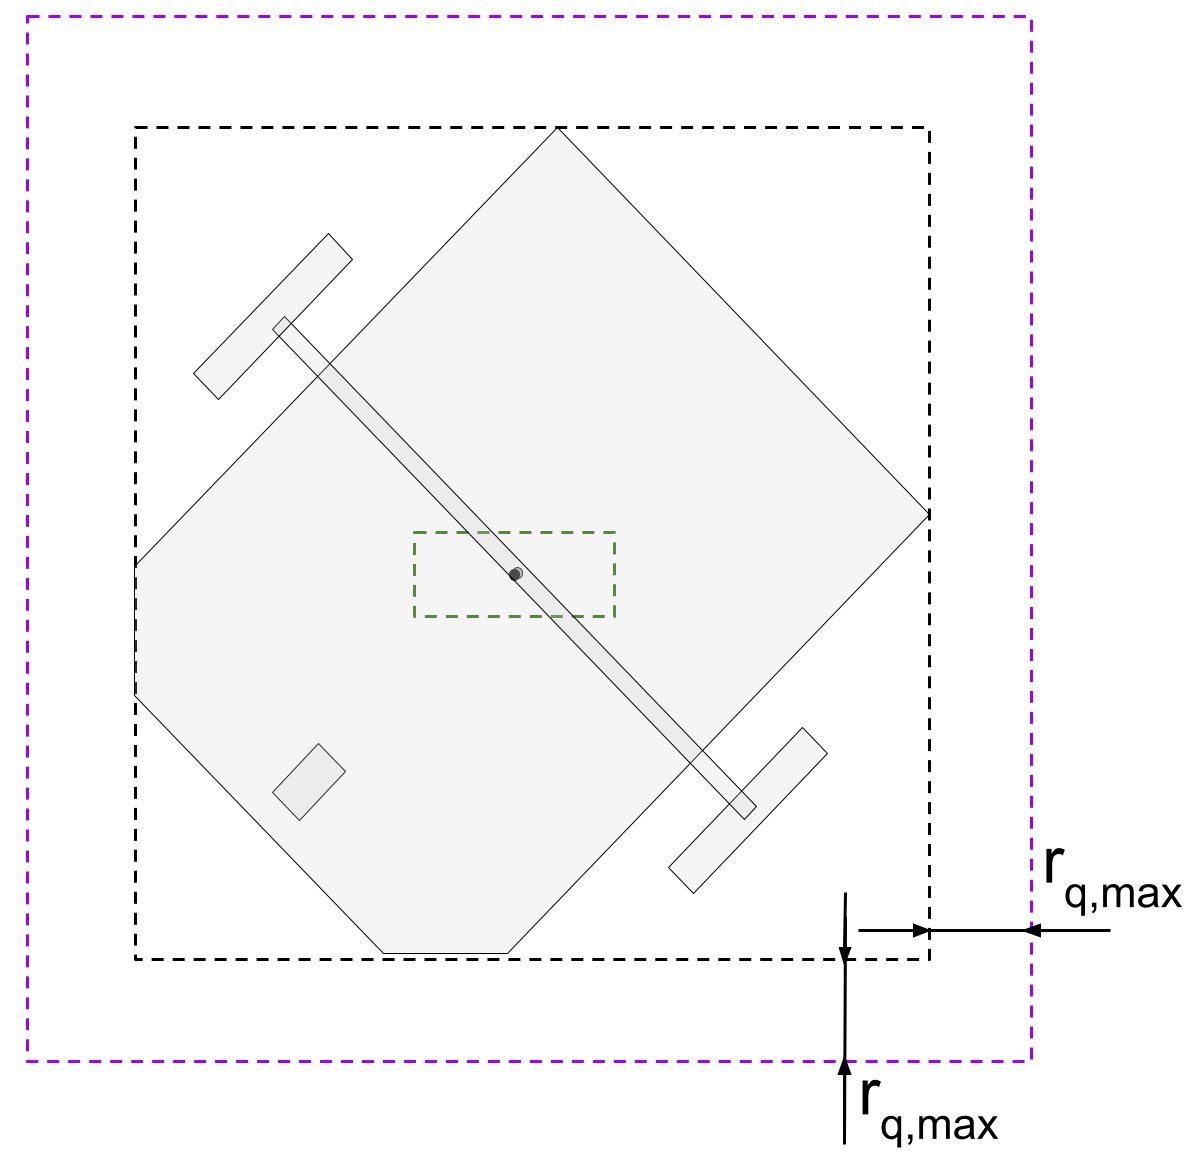
\includegraphics[width=\linewidth]{figures/samp/CC1.png}
%         \caption{}
%         \label{fig:CC1}
%     \end{subfigure}
%     % \hfill
%     \begin{subfigure}{0.4\textwidth}
%         \centering
%         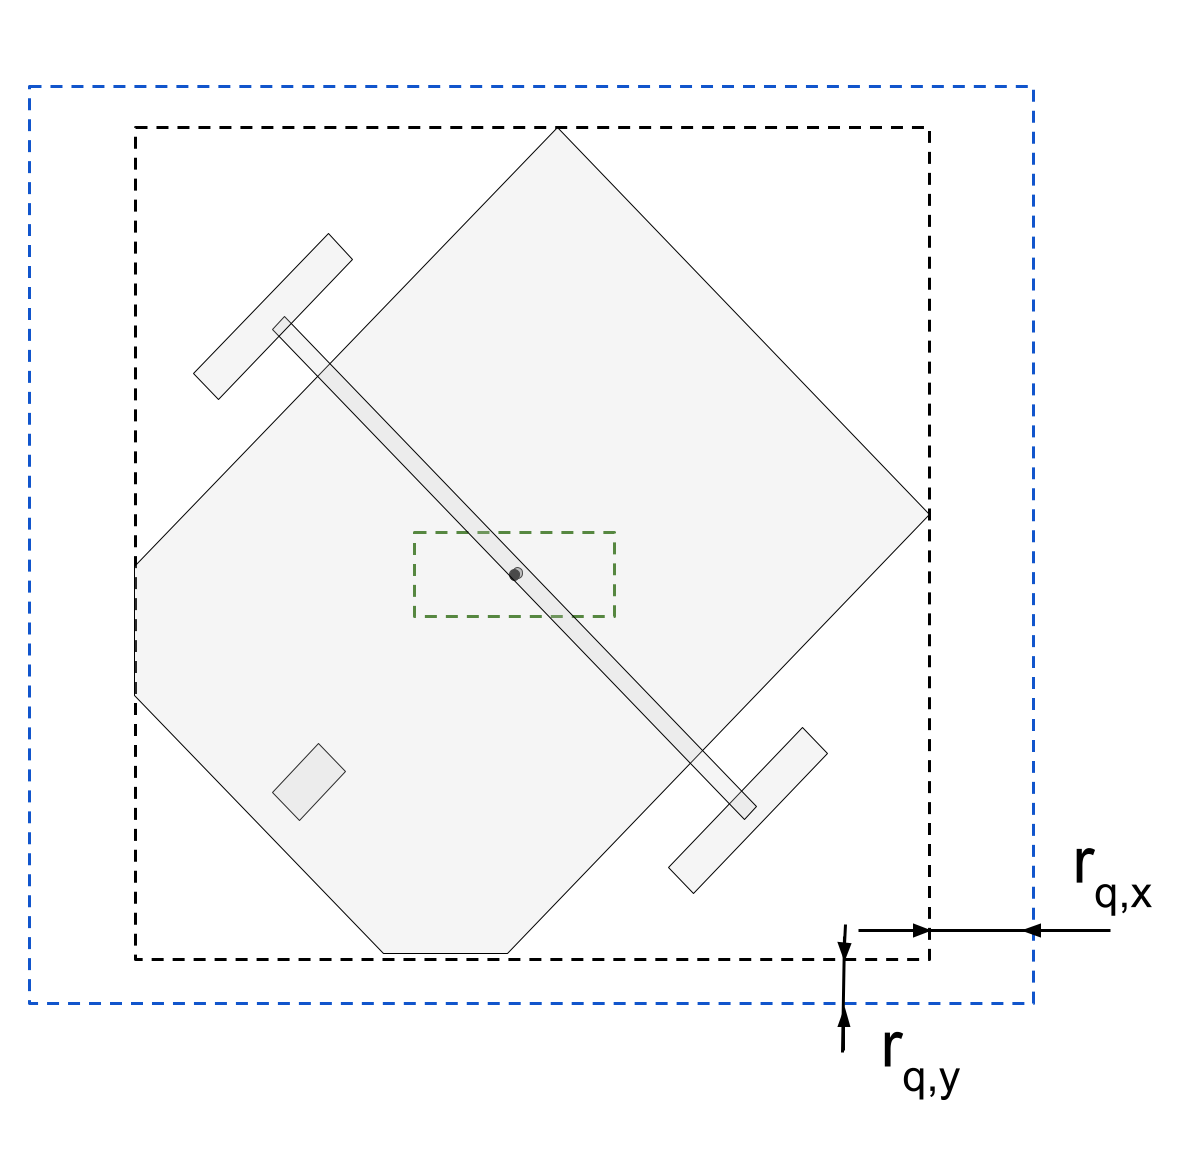
\includegraphics[width=\linewidth]{figures/samp/CC2.png}
%         \caption{}
%         \label{fig:CC2}
%     \end{subfigure}
    
%     % Row 2
%     \begin{subfigure}{0.4\textwidth}
%         \centering
%         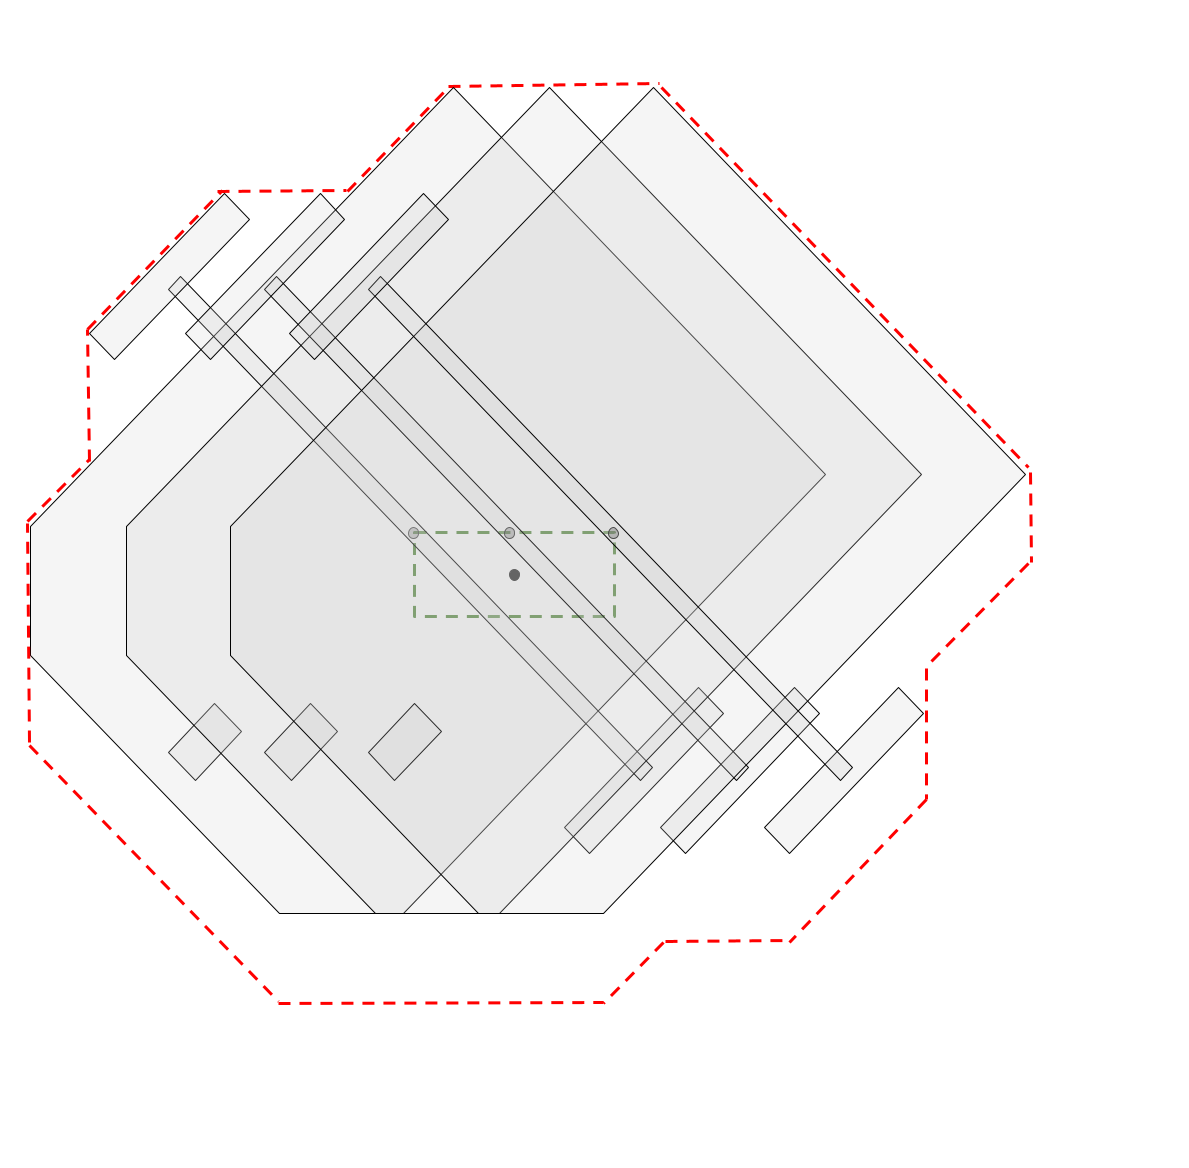
\includegraphics[width=\linewidth]{figures/samp/CC3.png}
%         \caption{}
%         \vspace{-0.3cm}
%         \label{fig:CC3}
%     \end{subfigure}
%     % \hfill
%     \begin{subfigure}{0.4\textwidth}
%         \centering
%         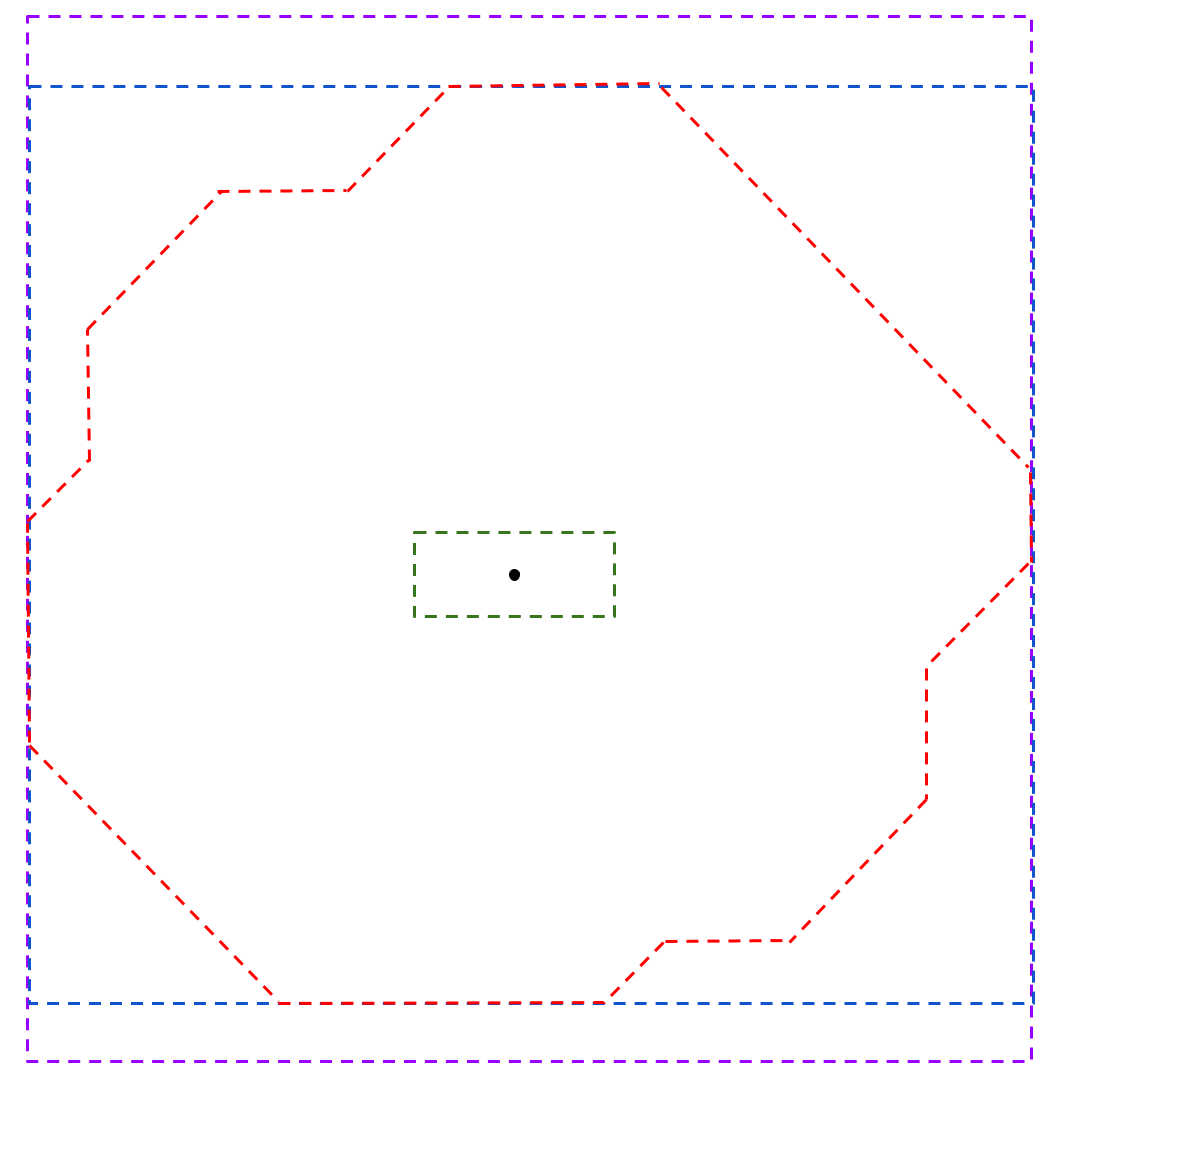
\includegraphics[width=\linewidth]{figures/samp/CCall.png}
%         \caption{}
%         \vspace{-0.3cm}
%         \label{fig:CCall}
%     \end{subfigure}

%     \caption{Figure showing the space covered by each of the three methods: (a) uniformly scaled AABB, (b) extended AABB, and (c) sampling-based approximation of the extended collision shape, for a differential drive robot with its associated uncertainty ellipsoid bounding box (green) based on computed uncertainty radii. Comparison of the three methods is shown in (d).}
%     \label{fig:CCmethods}
% \end{figure}

% These different approaches enable progressively more precise collision testing, from the first to the third method, as illustrated in the Figure~\ref{fig:CCall} that shows a comparison of the resulting tested collision shapes according to the aforementioned methods for the 2D differential drive robot.
% However, this increased accuracy comes at the cost of longer computational times, as noted earlier. 
% To quantify this, the mean running time of each method was evaluated based on 1.000 robust collision tests performed using the quadrotor model described in Section~\ref{sec:quad_model}. 
% The results indicate that the first method, which involves a simple distance check, has an average runtime of 3 microseconds. 
% The second method, which creates an extended uncertain AABB, takes 7 microseconds to compute. 
% Finally, the method that approximates the true extended collision shape requires 45 microseconds. 
% It is worth mentioning that this last approach involves 14 samples (each corner and the center of each face), and therefore, its runtime can be approximated as linear with respect to the number of samples, compared to a simple test.

% Finally, in this thesis, the second approach is used for robust collision checking, as it offers a more precise approximation of the extended collision shape with only a minor increase in computation time than the first approach. 
% However, the third approach is employed in the scenario presented in Section~\ref{sec:AOptim}, as it demands a higher level of collision accuracy.
% Although the methods employed in this thesis for robust collision checking rely on the uncertainty ellipsoid bounding box computed using Equation~\ref{eq:radius}, the tubes are represented by ellipsoids in the various figures of this manuscript for smoother visualization.

% \paragraph{Robust saturation checking}
% Then, in this manuscript, the feasibility check is not restricted to the aforementioned collision test, but it also verifies that the robot control inputs does not saturate.
% This test is performed by checking that the tube associated with each control input remains in its feasibility domain.
% An example of infeasible input for the quadrotor case is presented in Figure.\ref{fig:invalid_inputs}, where the tube (green) around the nominal control input of the first actuator (blue) exceeds the maximum allowed input (red).
% Note that this simple test is less costly than the robust collision checking one, it is therefore performed first by mean of computational efficiency. 

% \begin{figure} [htp]
%     \centering
%     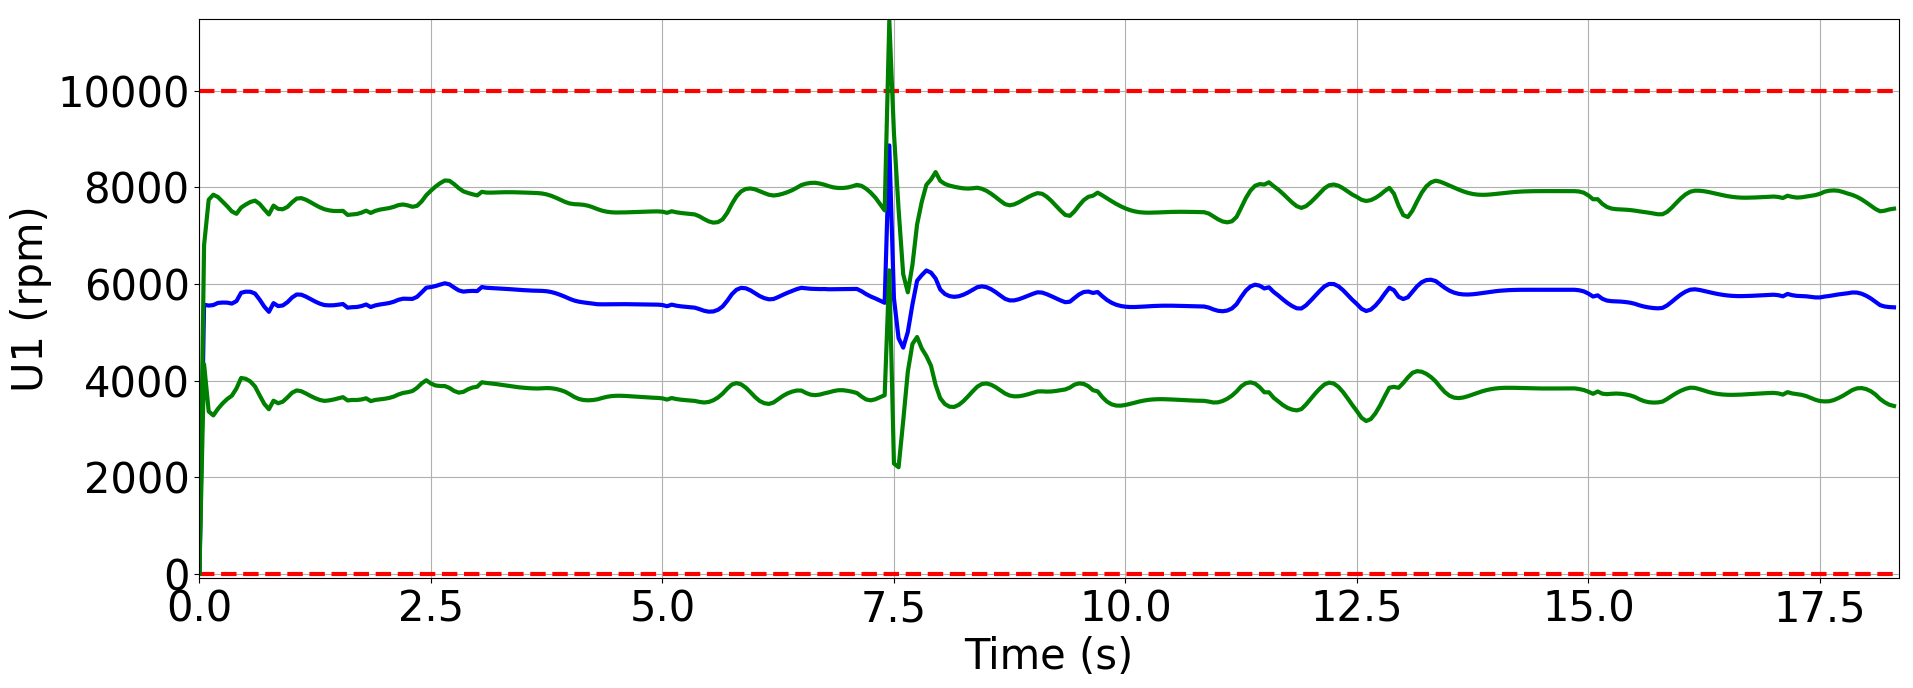
\includegraphics[width=0.8\linewidth]{figures/samp/Invalid_Inputs.png} 
%     \caption{Non-robust nominal control input profile for the first rotor of a quadrotor (blue) along a specified trajectory, depicted with its uncertainty tube (green) and the control input limits (red).}%
%     \label{fig:invalid_inputs}%
% \end{figure}

\section{Unified approach}\label{sec:unified}

This section present how the sensitivity matrices and resulting uncertainty tubes computation can be incorporated into any assymptotically-optimal tree planner in order to generate robust and sensitivity-optimal trajectories.  

\subsection{Overview}\label{sec:general_method}

\paragraph{Sampling-based motion planning with dynamic}

As shown in Section~\ref{sec:sensi_and_tubes}, the state/input sensitivity matrices (and resulting uncertainty tubes) are computed by forward integrating the set of \myglsentry{odes} presented by Equation~(\ref{eq:dyna}), Equation~(\ref{eq:ctrl}), and Equation~(\ref{eq:dyna_sensi}).
This computation is performed using the controller time step along a given desired trajectory.
In a sampling-based framework, this computation must be performed at each new extension to assess the trajectory cost and the associated uncertainty tubes for the robust feasibility check.
% Although the \myglsentry{odes} need to be solved at each controller time step, it is important to note that the robust feasibility check presented in Section~\ref{sec:robust_CC} can be conducted using a coarser time step.

Furthermore, in a sampling-based context, solving the \myglsentry{odes} from a set of non-zero initial conditions (e.g. $\bPi_0$, $\q^0$ etc.), denoted $S_0$, is required when an extension is made from a node that is not the root.
Therefore, after a feasible extension is made and the new node is added to the structure, the set of final conditions (e.g. $\bPi_F$, $\q^F$,  etc.), denoted $S_F$, must be embedded within the new node.
These conditions are then reused as initial conditions for future extensions.
Moreover, it is important to note that the initial conditions of a given node are determined by the trajectory from the root node. 
As a result, these initial conditions are specific to the parent node, making them applicable only in tree-based planners, where each node has exactly one parent.
Indeed, graph-based planners, such as \myglsentry{prm}~\cite{cPRM}, are unable to leverage such mechanisms due to their high degree of connectivity.
Additionally, note that, since dynamics are taken into account, the algorithms presented in this thesis utilize directed data structures (i.e., structures like directed trees that represent dependencies and directionality in motion).

\paragraph{Standard RRT*}

The vanilla \gls{rrtstar}~\cite{cRRTstar} is a widely used asymptotically optimal sampling-based planner that extends the standard \gls{rrt}~\cite{cRRT} algorithm by incorporating a rewiring step to iteratively improve the quality of the trajectories in the generated tree.
It achieves this by first optimally connecting the samples to the tree and then re-evaluating the connections between sampled nodes and their neighbors based on a cost metric. 
This process ensures that the tree progressively converges toward an optimal solution as the number of samples increases.
The \myglsentry{rrtstar} tree extension process and tree rewiring phase are illustrated in Figure~\ref{fig:rrtstar}.

\begin{figure} [htp]
    \centering
    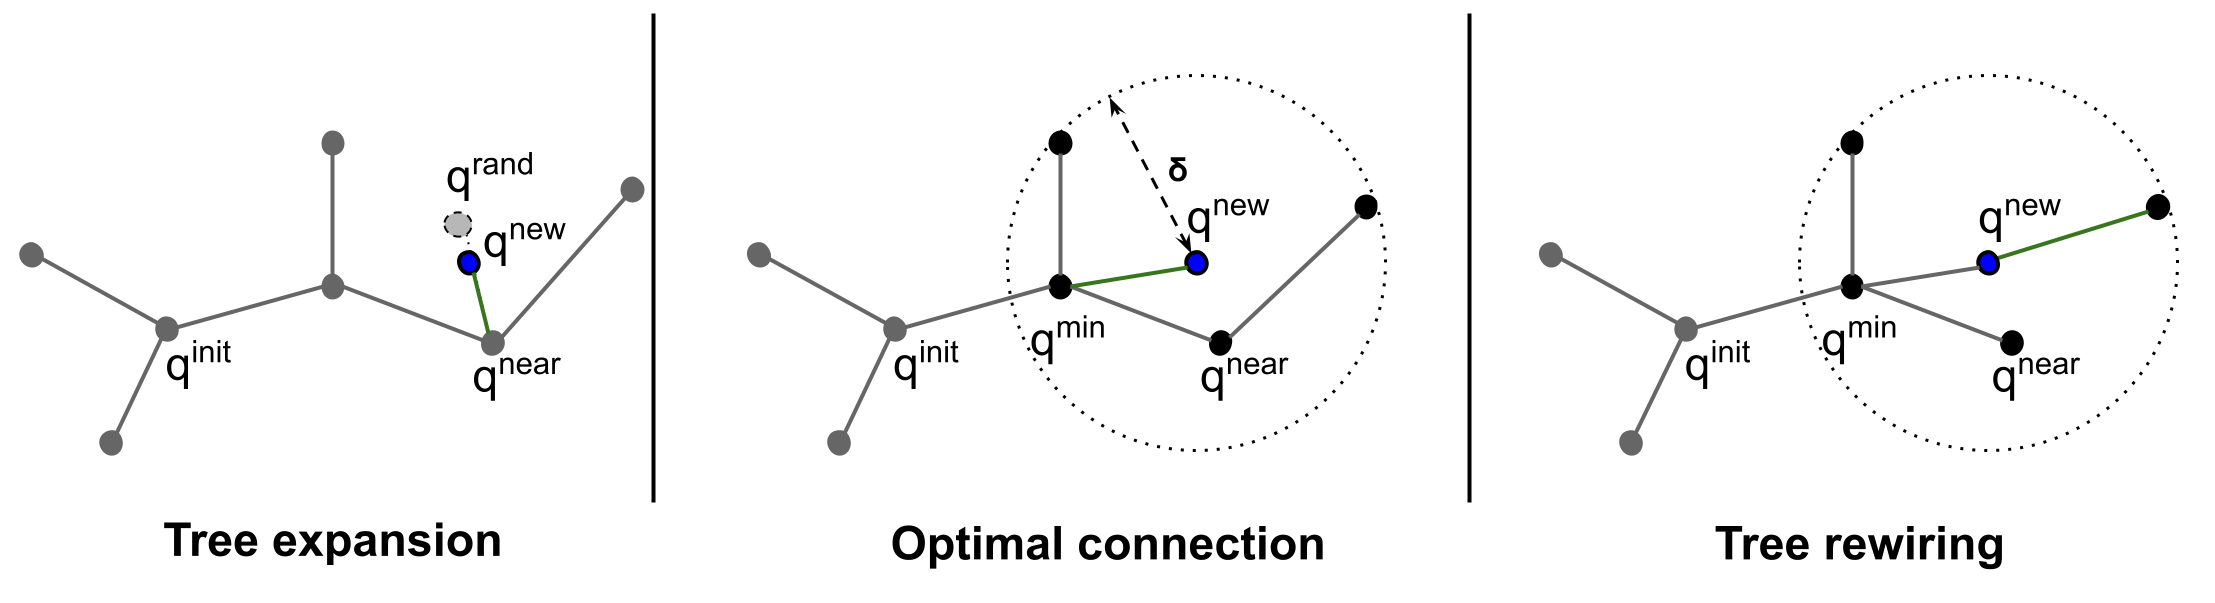
\includegraphics[width=0.95\linewidth]{figures/samp/rrtstar.png} 
    \caption{Illustration of the \myglsentry{rrtstar} tree extension procedure.
    The first phase (left) consists of extending the nearest node in the tree, $q^{near}$, towards a randomly sampled state,$q^{rand}$, in order to add a new collision-free state, $q^{new}$, to the tree.
    Then, an optimal connection phase is performed (middle), where the new node is optimally connected to the node with the minimum cost, $q^{min}$, from the start, within a neighborhood defined by a distance $\delta$.
    Finally, within this same neighborhood, a rewiring phase (right) is attempted to optimally reconnect the existing nodes if the cost of passing through the new state improves their current cost.}%
    \label{fig:rrtstar}%
\end{figure}

\paragraph{Standard SST*}

The standard \gls{sst*}~\cite{cSST} is another asymptotically optimal sampling-based planner that, unlike \myglsentry{rrtstar}, does not utilize a local planner but instead relies on system dynamics forward propagation.
This method grows a tree in the state space by employing Monte Carlo forward dynamic propagation to explore feasible trajectories by sampling control inputs.
To improve efficiency, \myglsentry{sst} employs a pruning mechanism that preserves only the locally optimal solutions, thanks to a witness and representative system as illustrated in Figure~\ref{fig:sst}.
This approach ensures that the planner focuses on promising regions of the state space, reducing redundant computations while maintaining theoretical guarantees of near-optimality. 
By combining these features, \myglsentry{sst} offers a powerful solution for kinodynamic motion planning in complex systems.

\begin{figure} [htp]
    \centering
    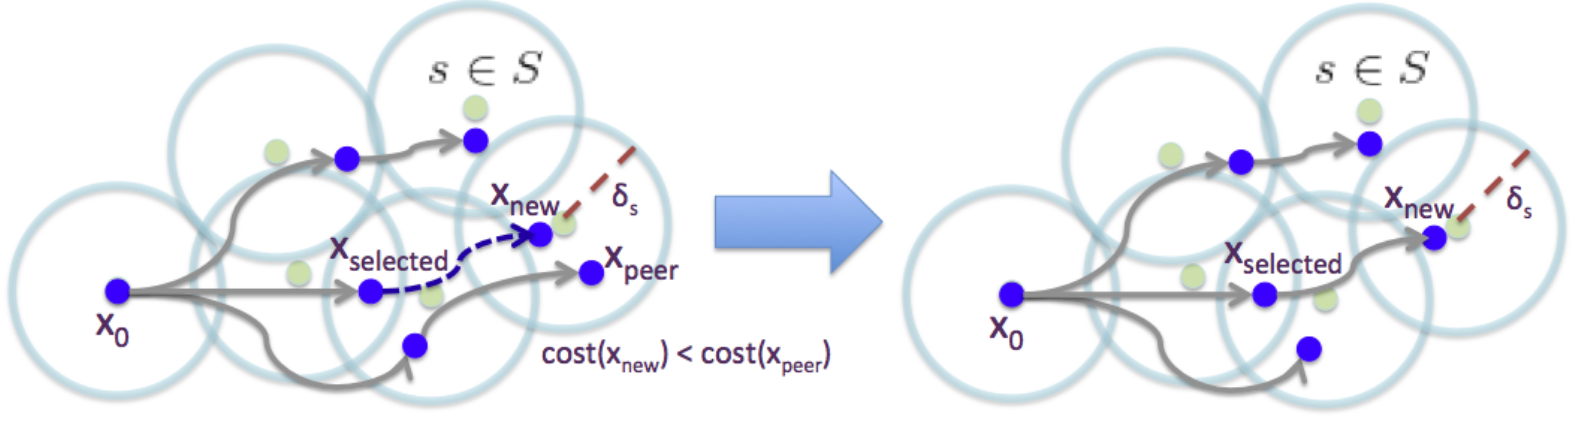
\includegraphics[width=0.95\linewidth]{figures/samp/sst.png} 
    \caption{Illustration of the \myglsentry{sst} tree extension procedure where white dots represent witnesses, and blue dots are current witnesses representative (i.e. the node with the best cost in the witness neighborhood) (extracted from~\cite{cSST}).
    Dynamic propagation from $x_{selected}$ generates a new node $x_{new}$, which has a better trajectory cost than its current witness representative node $x_{peer}$.
    In this case, $x_{peer}$ is pruned, and the newly propagated edge is incorporated into the tree as the new witness representative.
    If $x_{peer}$ had children with the lowest trajectory cost in their respective neighborhoods, $x_{peer}$ would remain in the tree but would no longer be considered for further propagation. 
    Inversely, if $x_{new}$ has a worse trajectory cost than $x_{peer}$, the old node $x_{peer}$ remains in the tree, and the propagation from $x_{selected}$ to $x_{new}$ is ignored.}%
    \label{fig:sst}%
\end{figure}

\subsection{Sensitivity-Aware Motion Planner (SAMP)}\label{sec:samp}

The following subsection describes how the concepts outlined above can be incorporated into different tree planners to develop robust, sensitivity-aware variants, generally referred to as \gls{samp}\footnote{It is important to note that none of the proposed variants are formally proven to be complete, as establishing completeness would require a separate proof for each variant and determining an upper bound for the first-order approximation of the tube.}.
Note that although the following sections of this chapter focus on asymptotically-optimal planner variants to generate globally sensitivity-optimal trajectories, the same principles can easily be applied to non-asymptotically optimal planners (see Chapter~\ref{chap:sampNN}), such as the standard \gls{rrt}.

For clarity in the pseudo-code, the temporal notation is omitted in this subsection. 
Thus, bold symbols refer to time-dependent vectors (e.g., $\q_d$ represents a desired trajectory, $\Rq$ stands for the uncertainty tube radii along a trajectory, etc.), while non-bold symbols represent instantaneous vectors (e.g., $q^{rand}$ denotes a random state, and $S_0$ represents the initial conditions of the \myglsentry{odes} at a given state vector, etc.).

\subsubsection{Sensitivity-Aware RRT* (SARRT*)}

\begin{algorithm}[htp]
    \caption{SARRT$^* [q^{init}, q^{goal}]$}\label{alg:SARRT*}
    \begin{algorithmic}[1]
        \State $T \gets$ InitTree$({q^{init}, q^{goal}});$
        \While{\textbf{not} StopCondition$(T, {q^{goal}})$}  
            \State $q^{rand} \gets $Sample()$;$
            \State $q^{nearest} \gets$ Nearest$(T,{q^{rand}});$
            \State $\q_d \gets$ LocalPlan$({q^{nearest}},{q^{rand}});$
            \State $S_0 \gets $GetNodeConditions$({q^{nearest}});$
            \State $\left \{\q_n, \u_n, \Rq, \Ru, S_F \right \}  \gets $SolveODEs$(\q_d, S_0);$
            \If {IsRobust$(\Rq,\Ru, \q_n, \u_n)$}
                \State $q^{min} \gets q^{nearest};$
                \State SetNodeConditions$({q^{rand}}, S_{F});$
                \State $Q^{near} \gets$ NearestNodes$(T,{q^{rand}});$
                \State RobustOptimalConnection$(T, Q^{near}, q^{rand}, q^{min});$
                \State RobustRewire$(T, Q^{near}, q^{min});$
            \EndIf
        \EndWhile
        \State \textbf{return} GetTrajectory$(T, q^{init}, q^{goal})$;
    \end{algorithmic}
\end{algorithm}

\begin{algorithm}[htp]
    \caption{RobustOptimalConnection$[T, Q^{near}, q^{rand}, q^{min}]$}\label{alg:RobustOptimalConnect}
    \begin{algorithmic}[1]
        \State $c^{min} \gets$ Cost$(q^{rand});$
        \For {each $q^{near} \in Q^{near}$}
            \State $\q_d \gets$ LocalPlan$(q^{near},q^{rand});$
            \State $S_0 \gets $GetNodeConditions$({q^{near}});$
            \State $\left \{\q_n, \u_n, \Rq, \Ru, S_F \right \}  \gets $SolveODEs$(\q_d, S_0);$
            \If {IsRobust$(\Rq,\Ru, \q_n, \u_n)$}
                \If {Cost$(q^{near}) + J(\q_d) < c^{min}$}
                    \State $q^{min} \gets q^{near}; c^{min} \gets$ Cost$(q^{near}) + J(\q_d);$
                    \State SetNodeConditions$({q^{rand}}, S_{F});$
                \EndIf
            \EndIf
        \EndFor
        \State AddNewNode$(T, {q^{rand}});$
        \State AddNewEdge$(T, {q^{min}}, {q^{rand}});$
    \end{algorithmic}
\end{algorithm}

\begin{algorithm}[htp]
    \caption{RobustRewire$[T, Q^{near}, q^{min}]$}\label{alg:RobustRewire}
    \begin{algorithmic}[1]
        \For {each $q^{near} \in Q^{near} \backslash \{q^{min}\}$}
            \State $\q_d \gets$ LocalPlan$(q^{rand}, q^{near});$
            \State $S_0 \gets $GetNodeConditions$({q^{rand}});$
            \State $\left \{\q_n, \u_n, \Rq, \Ru, S_F \right \}  \gets $SolveODEs$(\q_d, S_0);$
            \If {IsRobust$(\Rq,\Ru, \q_n, \u_n)$}
                \If {Cost$(q^{rand}) + J(\q_d) <$ Cost$(q^{near})$}
                    \State $q^{parent} \gets$ GetParent$(q^{near});$
                    \State RemoveEdge$(T, q^{parent}, q^{near});$
                    \State AddNewEdge$(T, q^{rand}, q^{near});$
                    \State SetNodeConditions$(q^{near}, S_{F});$
                    \State UpdateChildren$(T, q^{near});$
                \EndIf
            \EndIf
        \EndFor
    \end{algorithmic}
\end{algorithm}

The first implementation presented in Algorithm~\ref{alg:SARRT*} is a variant of the widely used \myglsentry{rrtstar}~\cite{cRRTstar}, denoted \gls{sarrt*} as a particular instance of \myglsentry{samp}.
The tree is initialized with the desired initial and goal robot states, $(q^{init}, q^{goal})$ (line 1), and the algorithm continues until a user-defined stopping criterion is met (line 2).
Such a criterion can include a maximum number of iterations, a maximum runtime, a cost convergence threshold, etc.

The first stage of the algorithm follows the same standard procedure as the vanilla \myglsentry{rrtstar}, including sampling a desired robot state $q^{rand}$ and finding its nearest neighbor $q^{nearest}$ in the tree structure (lines 3 and 4, respectively) using an efficient distance metric.
Then, a local planner (such as the ones presented in Section~\ref{sec:kinosplines} and Section~\ref{sec:dubins}) is employed to generate a desired local trajectory $\q_d$ that extends $q^{nearest}$ toward $q^{rand}$.
Note that if a maximum local distance is imposed, $q^{rand}$ is adjusted accordingly.
Next, as discussed in Section~\ref{sec:general_method}, the set of \myglsentry{odes} is solved (line 7) to compute the nominal trajectory $\q_n$, the nominal control inputs $\u_n$, and the uncertainty tubes $(\Rq, \Ru)$, utilizing the initial conditions $S_0$ (line 6).
A robust feasibility check is then conducted along the nominal trajectory and control inputs (line 8).
This test includes a robust collision check that accounts for the robot shape expansion due to uncertainty tubes along the state trajectory, as well as a robust verification that the control inputs do not saturate.
Remember that this test is carried out along the nominal values, as the uncertainty tubes are valid around them, as detailed in Section~\ref{sec:tubes}.
If the extension is feasible, the new node parent is temporarily set to $q^{nearest}$, and the final conditions $S_F$ are temporarily stored within $q^{rand}$ (line 9-10).

Next, to identify the optimal parent of $q^{rand}$, which is temporarily assigned to $q^{min}$, an additional search is conducted within a specified neighborhood $Q^{near}$ (line 11).
Such procedure, depicted in Algorithm~\ref{alg:RobustOptimalConnect}, starts by computing the cost of the unique trajectory from the root node to $q^{rand}$ (line 1).
Then, the optimal parent $q^{min}$ is set to the node in $Q^{near}$ that allows a robust extension while incurring the minimum cost to get to $q^{rand}$ (line 2-9).
Finally, the new node is inserted in the tree with its optimal parent (line 10-11).

Now that the optimal feasible extension is added to the tree, the \myglsentry{sarrt*} checks if any optimal rewiring can be performed using Algorithm~\ref{alg:RobustRewire}.
This rewiring phase checks, for each neighbor $q^{near}$ within $Q^{near}$, whether the trajectory from the root to $q^{near}$, passing through the newly added node $q^{rand}$, can be improved (lines 1-6).
In such case, the parent of $q^{near}$ is updated accordingly, and the final \myglsentry{odes} conditions $S_F$ are also modified (lines 7-10).
Finally, in contrast to the standard \myglsentry{rrtstar}, each child of the newly rewired node must be rechecked for robust feasibility, as their uncertainty tubes and control inputs may have changed due to the updated trajectory resulting from the rewiring (line 11).
Note that this final operation requires re-solving the \myglsentry{odes} for each child node.

\subsubsection{Sensitivity-Aware SST* (SASST*)}

It is important to note that a single iteration of \myglsentry{sarrt*} presented above requires solving the set of \myglsentry{odes} multiple times which leads to a prohibitive computation time per iteration as shown in Section~\ref{sec:samp_simu}.
To mitigate this impact, this subsection proposes a robust sensitivity-aware variant of the \gls{sst*}~\cite{cSST}, denoted \gls{sasst*} as a particular instance of \myglsentry{samp}. 

The \myglsentry{sst*} algorithm has two key features: it reduces the number of collision checks to just one per iteration and uses Monte Carlo propagation to sample the control input space and perform forward dynamic propagation, eliminating the need for a local planner.
However, since this thesis uses the system closed-loop dynamics for sensitivity computation rather than open-loop Monte Carlo propagation, the latter is replaced by a local planner.

The \myglsentry{sasst*} variant, detailed in Algorithm~\ref{alg:SASST*}, operates as follows:
\begin{itemize}
    \item It first performs metrics and tree initialization (line 1-4) by splitting it into two subsets: $V_{active}$ and $V_{inactive}.$
    Nodes in $V_{active}$ are those with the optimal trajectory cost from the root within their local neighborhoods. 
    In contrast, nodes in $V_{inactive}$ while suboptimal in trajectory cost, are preserved in the tree to maintain connectivity, as they have children with better trajectory costs in their respective neighborhoods. 
    \item To define local neighborhoods, the algorithm leverages an auxiliary set of states called "witnesses," denoted as $W$ (line 5). 
    Each witness $w \in W$ is associated with a single representative node in the tree, stored in the $w.rep$ field of the witness (line 6).
    This representative node corresponds to the trajectory with the lowest cost from the root within a distance $\delta_s$ of the witness $w$.
    Any nodes within the $\delta_s$-neighborhood of $w$ that have a higher trajectory cost than $w.rep$ are removed from the active set $V_{active}$.
    \item Then, until a user defined criterion is met, the algorithm performs for N iterations:
    \begin{enumerate}
        \item A best-first selection that samples a random state from the state space and finds the best node in terms of cost from the root within a distance of $\delta_{BN}$ in the active set of the tree. 
        This node, referred as $q^{selected}$, represents the state to be propagated (line 9).
        \item Then, instead of the original Monte Carlo propagation, a random state $q^{rand}$ is sampled within a maximum distance of $q^{selected}$ (line 10), analogous to sampling a control input and propagation duration in the vanilla algorithm.
        The local trajectory connecting the two state is computed (line 11) and, as discussed in Section~\ref{sec:general_method}, the set of \myglsentry{odes} is solved (line 12-13) before performing a robust feasibility check (line 14).
        \item If the local trajectory is robustly feasible, the set $W$ is used by the IsNodeLocallyTheBestSST procedure (line 15) to check whether the newly sampled state $q^{rand}$ dominates the $\delta_s$-neighborhood of its closest witness and to update the witness set $W$ accordingly.
        \item Then, the sample is added to the tree (line 16-17), and the sets of active and inactive nodes are updated.
        Nodes that no longer belong to any of these sets are pruned (line 18).
    \end{enumerate}
    \item Finally, after the N iterations, if the stopping criterion is not met, the hyperparameters of the algorithm are updated (line 19-21).
    These parameters are responsible for the algorithm asymptotic optimality and convergence. 
    The algorithm gradually reduces the radii $\delta_s$ and $\delta_{BN}$, enabling it to explore new homotopic classes over time.
\end{itemize}

Note that in this implementation the \myglsentry{odes} need to be solved only once per iteration compared to the \myglsentry{sarrt*} implementation.

\begin{algorithm}[htp]
    \caption{SASST$^* [q^{init}, q^{goal}, N_0, \delta_{BN,0}, \delta_{s,0}, \xi]$}\label{alg:SASST*}
    \begin{algorithmic}[1]
        \State $j \gets 0; N \gets N_0;$
        \State $\delta_{s} \gets \delta_{s,0}; \delta_{BN} \gets \delta_{BN,0};$
        \State $V_{active} \gets \{q^{init}, q^{goal}\}, V_{inactive} \gets \emptyset;$
        \State $T \gets$ InitTree$(V_{active}, V_{inactive});$
        \State $w_0 \gets q^{init}, w_G \gets q^{goal}, W \gets \{w_0, w_G\};$
        \State $w_0.rep \gets q^{init}, w_G.rep \gets q^{goal};$
        \While{\textbf{not} StopCondition$(T, {q^{goal}})$}  
            \For{N iterations}
                \State $\{q^{selected}, q^{rand}\} \gets $BestFirstSelectionSST$(V_{active}, \delta_{BN});$
                \State $q^{rand} \gets$ Sample$(q^{selected}, d_{max});$
                \State $\q_d \gets$ LocalPlan$({q^{selected}},{q^{rand}});$
                \State $S_0 \gets $GetNodeConditions$({q^{selected}});$
                \State $\left \{\q_n, \u_n, \Rq, \Ru, S_F \right \}  \gets $SolveODEs$(\q_d, S_0);$
                \If {IsRobust$(\Rq,\Ru, \q_n, \u_n)$}
                    \If{IsNodeLocallyTheBestSST$(q^{rand}, W, \delta_s)$}
                        \State $V_{active} \gets V_{active} \cup \{q^{rand}\};$
                        \State AddNewEdge$(T, q^{selected}, q^{rand});$
                        \State PruneDominatedNodesSST$(q^{rand}, V_{active}, V_{inactive});$
                    \EndIf
                \EndIf
            \EndFor
            \State $\delta_s \gets \xi\delta_s; \delta_{BN}\gets\xi\delta_{BN};$
            \State $j \gets j+1;$
            \State $N \gets (1+$log $j)\xi^{-(d+1)j}N_0;$
        \EndWhile
        \State \textbf{return} GetTrajectory$(T, q^{init}, q^{goal})$;
    \end{algorithmic}
\end{algorithm}

\subsection{Simulation results}\label{sec:samp_simu}

This subsection presents the results of trajectory planning using the previously discussed variants, evaluated based on computation time, and robustness for the two systems introduced in Chapter~\ref{chap:models}.
To assess the impact of planning robust, globally sensitivity-optimal trajectories, both \myglsentry{sarrt*} and \myglsentry{sasst*} are compared with their respective non-robust vanilla versions, which focus on optimizing trajectory length.
The objective of this subsection is to quantify the ability of the proposed variants to generate robust solutions, and to evaluate the impact of solving \myglsentry{odes} multiple times within a sampling-based framework.
All planner implementations are performed using the \gls{ompl}~\cite{cOMPL}, and collision detection is performed using the widely used C implementation of PyBullet~\cite{cBullet}.
Recall that this robust feasibility check is performed not only in the state space but also in the control input space, as illustrated by Figure~\ref{fig:invalid_inputs}.
The \myglsentry{odes} are implemented using the JiTCODE~\cite{cJit} module which converts the equations to be integrated into C-compiled code.
The Euler integrator is then used to solve each ODE and take advantage of this compiled function.
Although the Euler method is less accurate than a Runge-Kutta 4-based method (e.g., dopri5), it is chosen because the uncertainty tubes are already an approximation, and faster predictions are preferred over higher accuracy in this context.

\begin{figure} [htp]
    \centering
    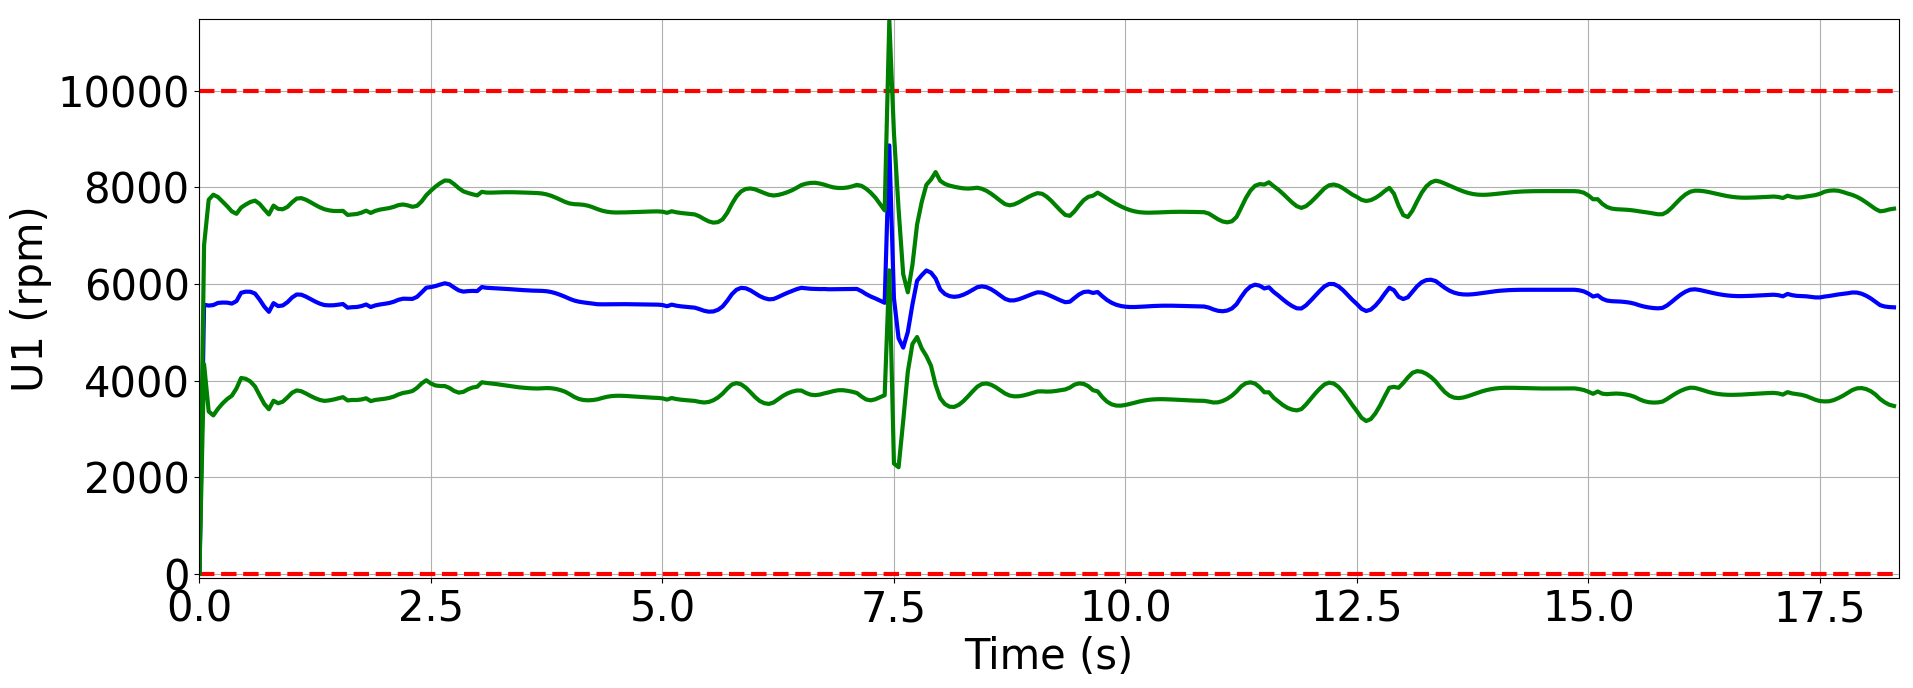
\includegraphics[width=0.8\linewidth]{figures/samp/Invalid_Inputs.png} 
    \caption{Non-robust nominal control input profile for the first rotor of a quadrotor (blue) along a specified trajectory, depicted with its uncertainty tube (green) and the control input limits (red).}%
    \label{fig:invalid_inputs}%
\end{figure}

\subsubsection{Cost function}\label{sec:sensi_cost}

First, generating a sensitivity-optimal trajectory requires identifying an appropriate sensitivity-based cost function.
The approaches in~\cite{cPi, cTh} proposed leveraging the Frobenius norm of the sensitivity matrices (Equation~\ref{eq:sensi}).
However, this formulation does not exploit the available information on the uncertainty ranges, $\delta \p$.

Therefore, in this work the largest eigenvalue of the kernel matrix $\bPi(t) \W \bPi(t)^T$ is considered as \emph{sensitivity norm}, since this represents the largest (worst-case) deviation in the state space. 
In particular, letting $\lambda_i(t)$ be the eigenvalues of $\bPi(t) \W \bPi(t)^T$, a smooth approximation of the $\max(\cdot)$ operator is performed with the $p$-norm:
\begin{equation}
    \lambda_{max}(t)\approx \left(\sum \lambda_{i}(t)^p\right)^{1/p}.
\end{equation} 

However, such function is neither additive (i.e., considering two desired trajectories ($\q_{d,1}(t), \q_{d,2}(t)$), the cost of their concatenation $c(\q_{d,1}(t)|\q_{d,2}(t)) \neq c(\q_{d,1}(t)) + c(\q_{d,2}(t))$), nor monotonic as depicted in Figure~\ref{fig:monotonic}.
Therefore, it is unsuitable for global optimization using sampling-based motion planners like~\cite{cRRTstar, cSST}, since they require additive and monotonic objective functions.
The total cost function $c(\q_d(t))$ for a desired trajectory $\q_d(t)$ is then defined considering its integral along the desired trajectory s.t.:
\begin{equation} \label{eq:cost_function}
    c(\q_d(t))=\int_{t_{0}}^{t_{f}}\lambda_{max}(\tau)d\tau.
\end{equation}
Minimization of this cost will minimize the largest deviation of the state tube along the whole motion.

\begin{figure} [htp]
    \centering
    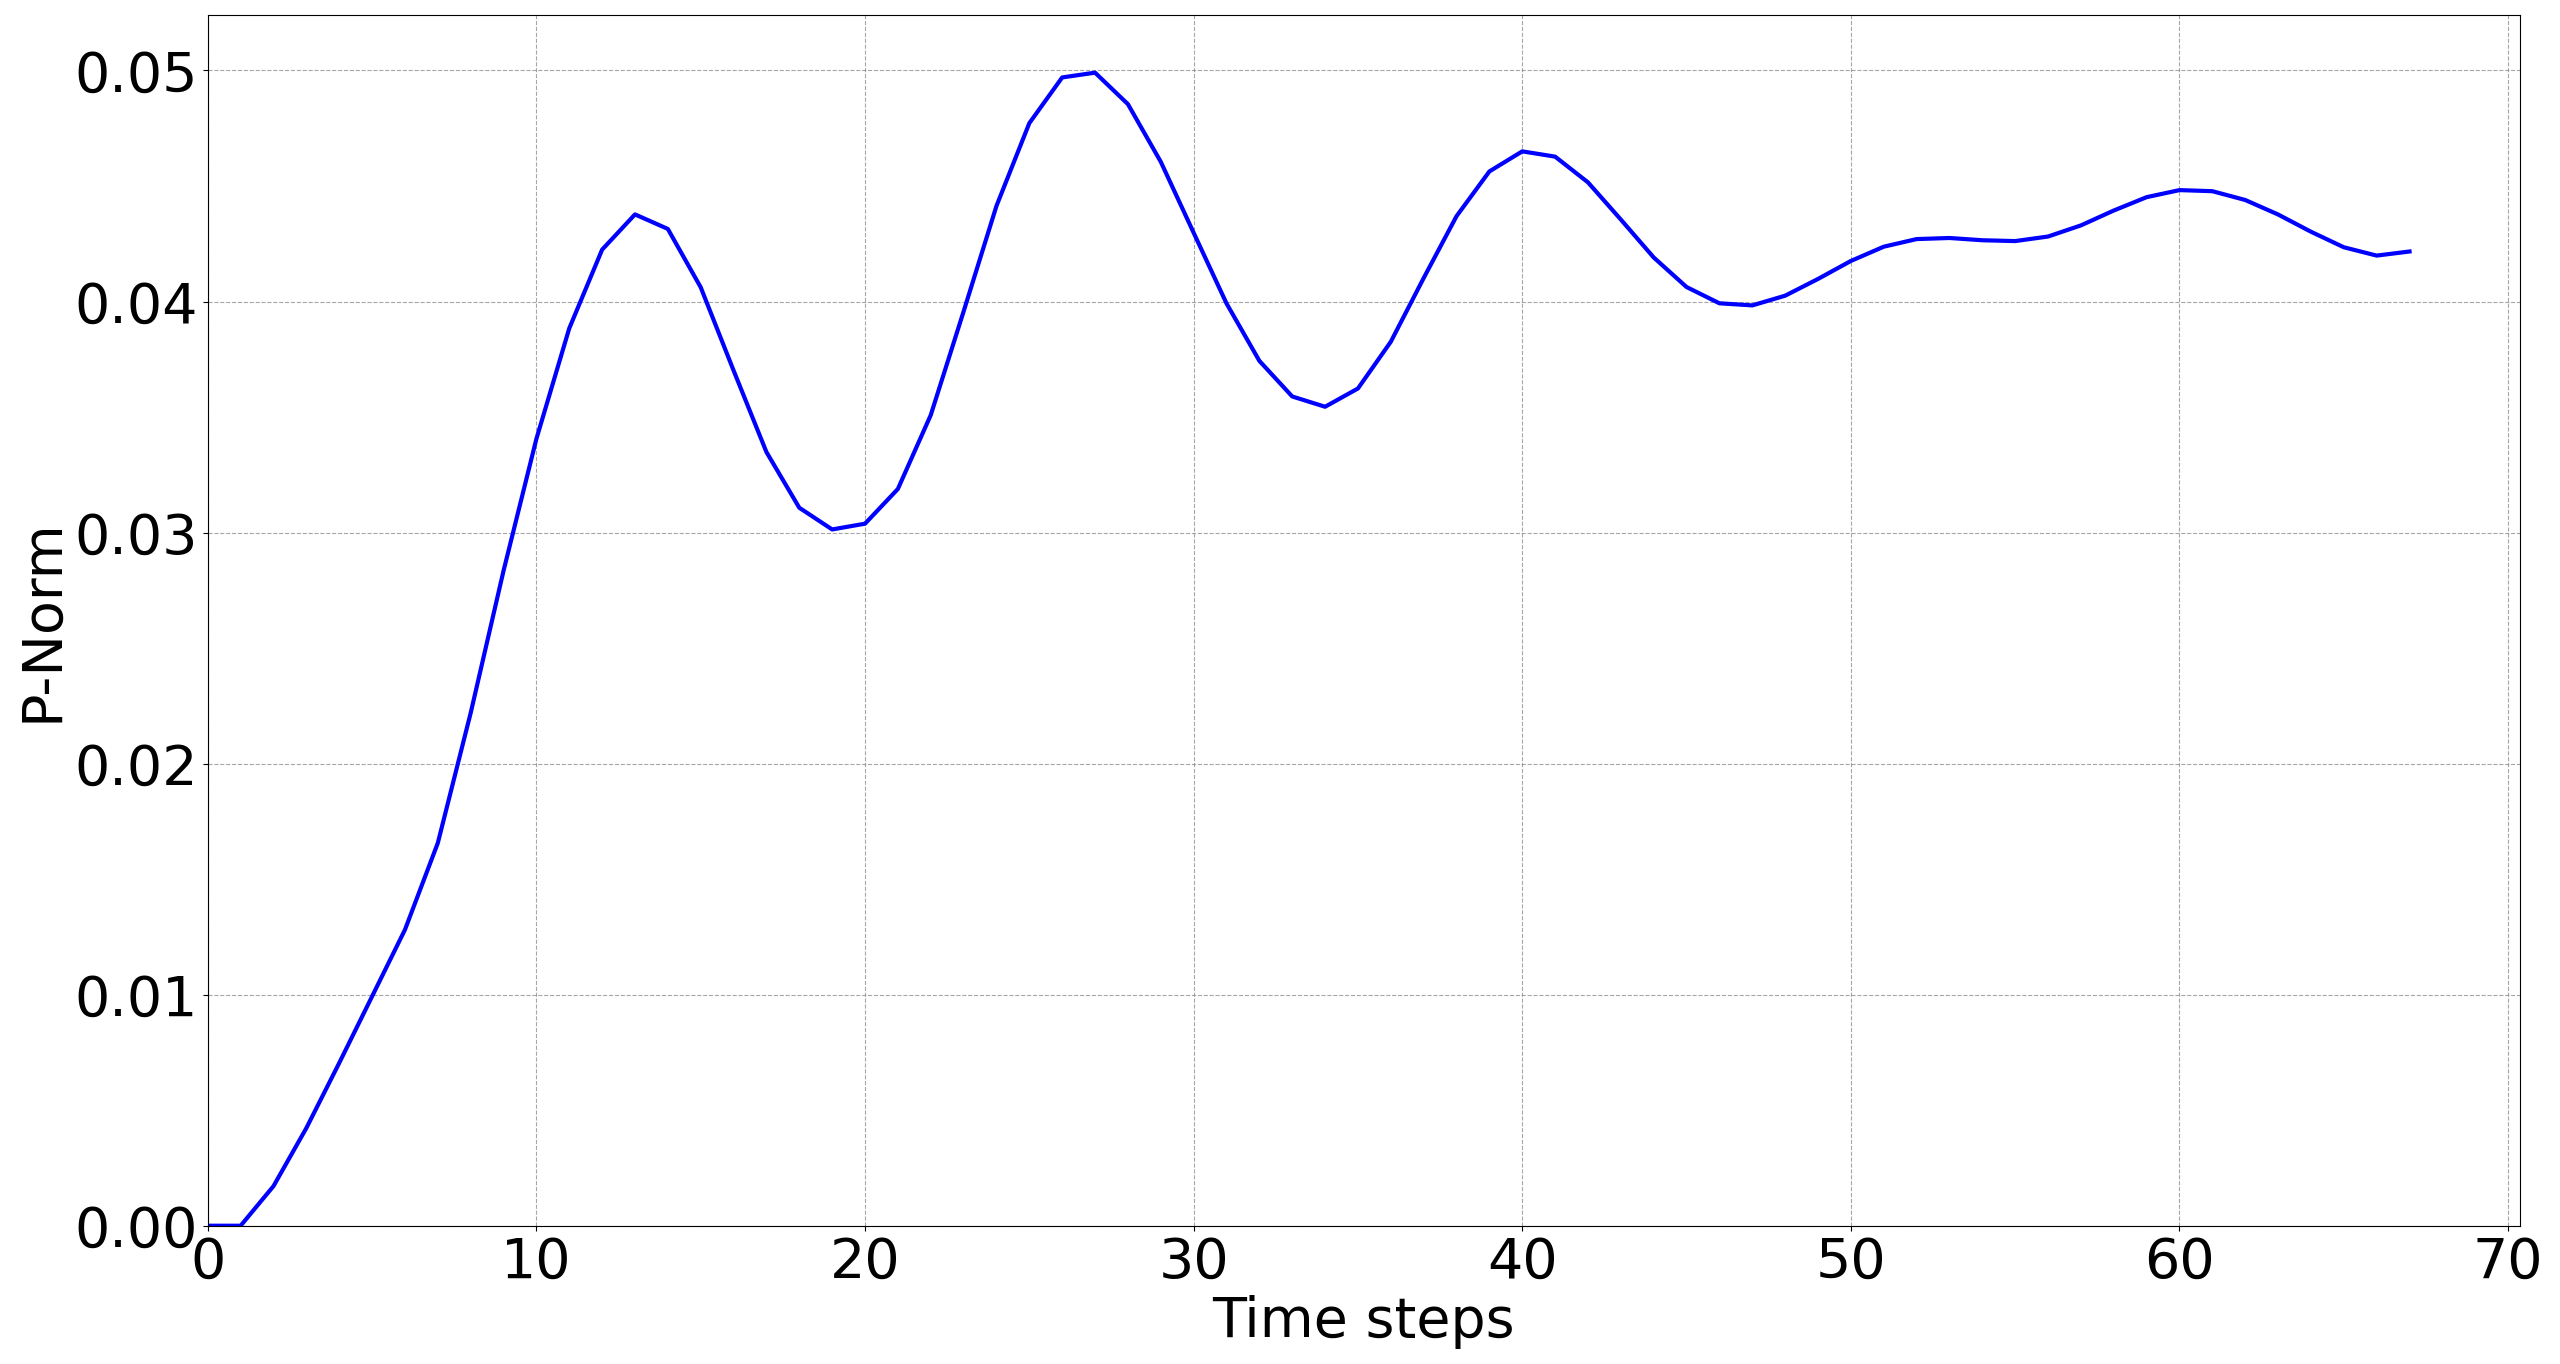
\includegraphics[width=0.7\linewidth]{figures/samp/non_monotoic.png} 
    \caption{Non monotonic p-norm profile along a 70-state trajectory for a quadrotor example.}%
    \label{fig:monotonic}%
\end{figure}

\subsubsection{Differential drive robot}

\paragraph{Robot setup}

This subsection presents results for the differential drive robot model depicted in Section~\ref{sec:unic_model}, with the following set of uncertain parameters $\p = [r, \, d]^T \in \mathbb{R}^{2}$.
The nominal value vector is set to $\p_n = [0.1m, \, 0.4m]^T$, with an associated uncertainty range of $\delta\p = [3\%, \, 3\%]^T$, representing the percentage deviation from their corresponding nominal values.
Therefore, in this differential drive robot application, $\bPi \in \mathbb{R}^{3\times2}$, $\bPixi\in \mathbb{R}^{3\times2}$, and $\bTheta \in \mathbb{R}^{2\times2}$.
As a result, the computations necessary to find the uncertainty tubes involve solving 16 \myglsentry{odes}.
The uncertainty tubes considered for this application are defined as $\Rq = [r_x, \, r_y]^T \in \mathbb{R}^2$, representing the uncertainty tubes along the x,y-axes of the state respectively, and $\Ru = [r_{u1}, \, r_{u2}]^T \in \mathbb{R}^2$, representing the uncertainty tubes along the two control input space axes ($\omega_r$ and $\omega_l$).
The controller gains are set to $\k_c = [1.5, \, 8.0, \, 0.2]^T$, and the control inputs limits are set to $\u_{max} = [60, \, 60]^T$, corresponding to the maximum speed of the two wheels expressed in rad.s$^{-1}$.

\paragraph{Planning setup}

Remind that the local planning method used is the Dubins path planner (see Section~\ref{sec:dubins}) with $v_{magn} = 1.0 m.s^{-1}$. 
Using the true cost-to-go as the distance metric is known to be computationally inefficient. 
However, as the cost of Equation~(\ref{eq:cost_function}) is strongly correlated to the trajectory length through the integral term, the length of the Dubins curves is used as the distance function heuristic. 

The hyperparameters for \myglsentry{sasst*} are selected based on the recommendations in~\cite{cSST}, with the following values: $N_0 = 10000$, $\delta_s = 0.5$, $\delta_{BN} = 1$, and $\xi = 0.9$.
For the maximum local distance, $d_{max}$ is set to 1.0.

The standard \myglsentry{ompl} \myglsentry{rrtstar} implementation typically defines a maximum local distance as a fraction of the state space maximum extent.
This approach can lead to excessively long trajectories, especially for large state space when two sampled states are far apart.
These trajectories frequently fail the robust feasibility check, leading to significant computational effort spent on computing uncertainty tubes only to detect early infeasibility. 
This inefficiency, resulting from highly constrained problems, slows down tree growth.
To address this, and following the approach used in the original \myglsentry{ompl} implementation, a fixed maximum distance is introduced for local trajectories. 
This adjustment does not compromise the algorithm properties, as longer trajectories can still be formed by chaining several shorter local trajectories. 
While this approach requires more iterations to ensure adequate space coverage and cost convergence, it results in more efficient tree growth under robustness constraints, as illustrated in Figure~\ref{fig:unic_tree}.
Note that the choice of this maximum local distance is critical for the applicability of the methods proposed in Chapter~\ref{chap:NN} and Chapter~\ref{chap:sampNN}.

Consequently, throughout this thesis, a maximum local trajectory length of 1.0 (meters or seconds according to the local planner used) is also applied to the proposed \myglsentry{sarrt*} and \gls{sarrt} (see Chapter~\ref{chap:sampNN}) variants.

Finally, all algorithms use a time step of 0.05s for the solving the \myglsentry{odes} and to perform the robust feasibility checks, and the algorithms stopping criterion is defined by a cost convergence threshold of 5\%.

\begin{figure} [htp]
    \centering
    \subfloat[\centering Fraction of the maximum space extent \myglsentry{rrtstar}]{{\includegraphics[width=0.4\linewidth]{figures/samp/rrtstar_unbounded.png} }}%
    \subfloat[\centering Fixed \myglsentry{rrtstar}]{{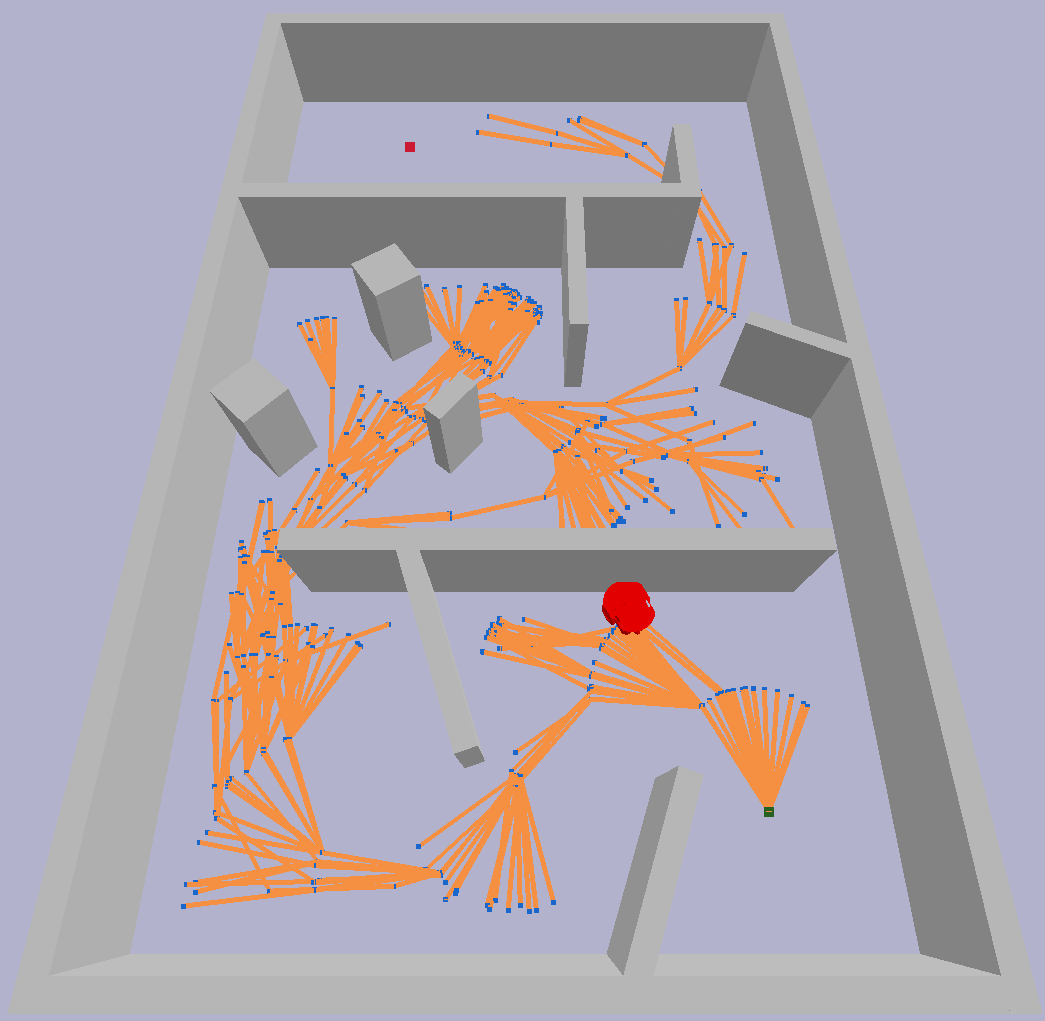
\includegraphics[width=0.4\linewidth]{figures/samp/rrtstar_bounded.png} }}%
    \\
    \subfloat[\centering Fraction of the maximum space extent \myglsentry{sarrt*}]{{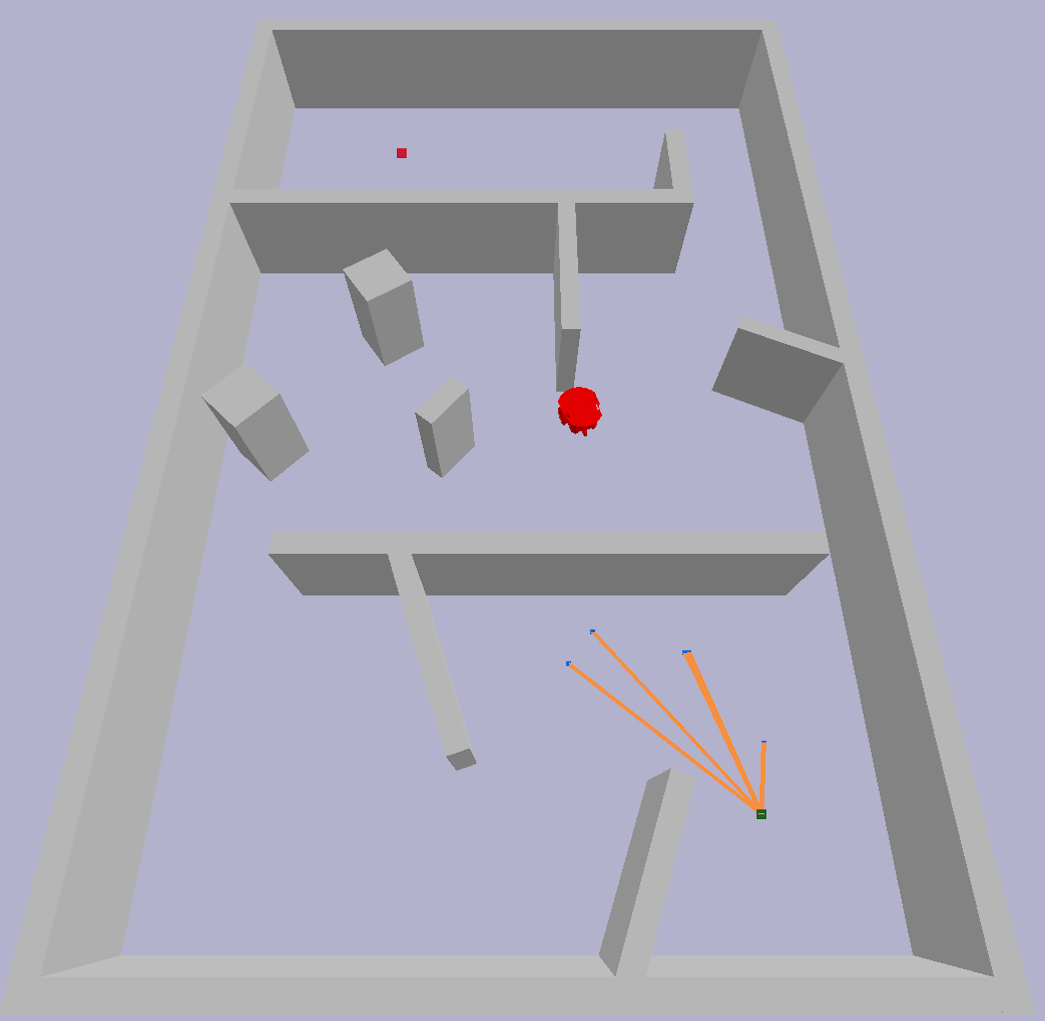
\includegraphics[width=0.4\linewidth]{figures/samp/sarrtstar_unbounded.png} }}%
    \subfloat[\centering Fixed \myglsentry{sarrt*}]{{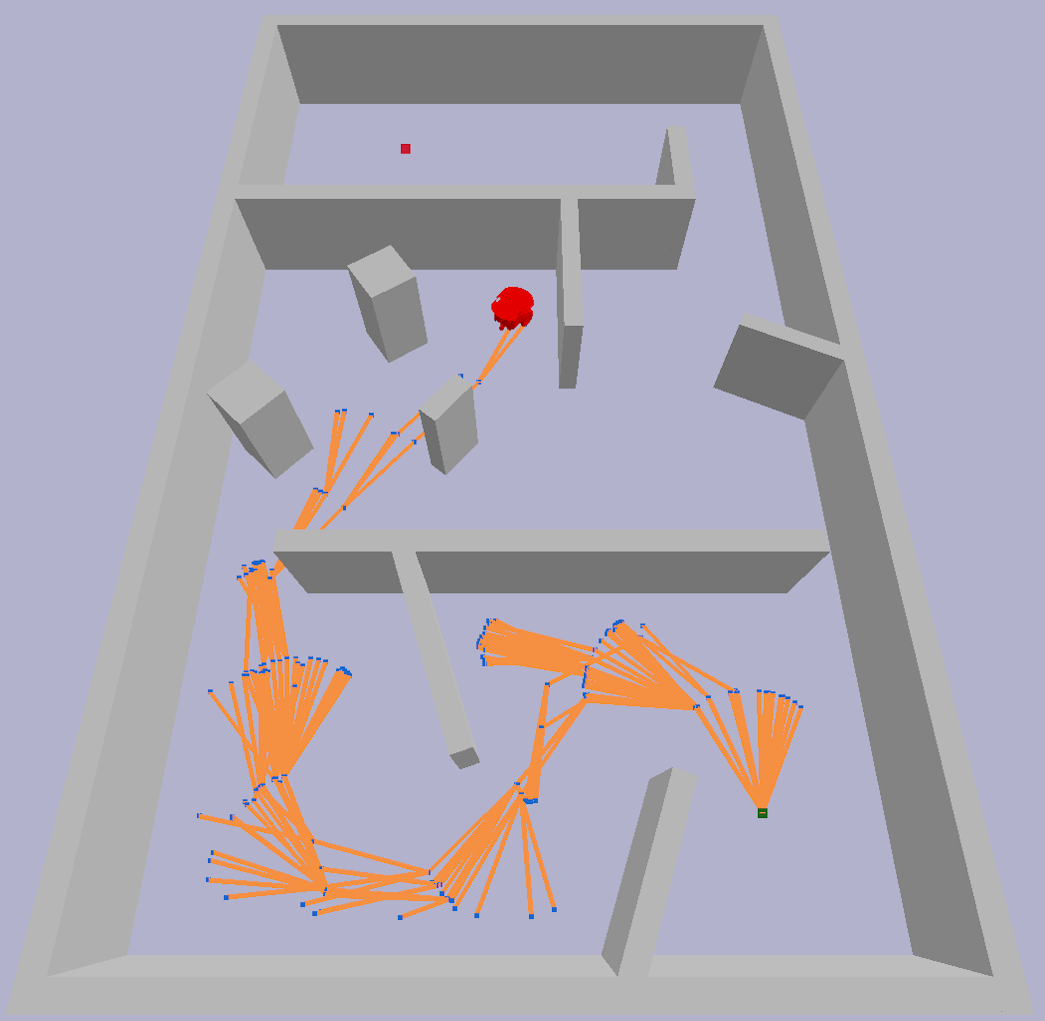
\includegraphics[width=0.4\linewidth]{figures/samp/sarrtstar_bounded.png} }}%
    \caption{Snapshot after 2.000 iterations of the trees generated by: (a) the \myglsentry{rrtstar} with a fraction of the maximum space extent as maximum local trajectory length, (b) \myglsentry{rrtstar} with fixed maximum local trajectory length, (c) the \myglsentry{sarrt*} with a fraction of the maximum space extent as maximum local trajectory length, and (d) the \myglsentry{sarrt*} with fixed maximum local trajectory length for the differential drive robot.
    Note that the local trajectories (in orange) are represented as linear segments only for visualization purposes.}%
    \label{fig:unic_tree}%
\end{figure}

\paragraph{Results}

\begin{table*}[t!]
    \centering
    \begin{tabular}{l|llll|}
    \cline{2-5}
        & \multicolumn{1}{c|}{RRT$^{*}$} & \multicolumn{1}{c|}{SARRT$^*$} & \multicolumn{1}{c|}{SST$^*$} & \multicolumn{1}{c|}{SASST$^*$} \\ \hline
    \multicolumn{1}{|c|}{Success (\%)} & \multicolumn{1}{c|}{3.3} & \multicolumn{1}{c|}{\textbf{100.0}}  & \multicolumn{1}{c|}{17.3}  &  \multicolumn{1}{c|}{\textbf{100.0}}   \\ \hline
    \multicolumn{1}{|c|}{Plan time (s)} & \multicolumn{1}{c|}{952 $\pm$ 201}   & \multicolumn{1}{c|}{4145 $\pm$ 639} & \multicolumn{1}{c|}{819 $\pm$ 155}  &   \multicolumn{1}{c|}{2148 $\pm$ 320}  \\ \hline
    \end{tabular}
    \caption{
    \label{tab:samp_unicycle}
    Average planning time and success rate (no crash) of the simulated motions planned by \myglsentry{rrtstar}, \myglsentry{sarrt*}, \myglsentry{sst*}, and \myglsentry{sasst*} over 10 plans and 30 simulations per plan, for the differential drive robot.}
\end{table*}

Table~\ref{tab:samp_unicycle} shows comparative results averaged for each planner over 10 trajectories and 30 simulations with uncertain parameters. 
The perturbations are uniformly sampled within an ellipsoid with semi-axis defined by $\delta \p$ as explained in Section~\ref{sec:tubes}.

First note that \myglsentry{sarrt*}, and \myglsentry{sasst*} variants have a significantly greater robustness compared to their respective standard, non-robust implementations.
This robustness is also illustrated in Figure~\ref{fig:robust_unic}, where the vanilla \myglsentry{rrtstar} is able to find the shortest solution which pass through a narrow corridor, however, this solution is not robust to the presence of uncertain parameters, leading to a poor robustness.
On the other hand, the \myglsentry{sarrt*}, is able to find the shortest trajectory under robust constraints, leading to a 100\% success rate.
It is important to note that this success rate is assessed based on both robust collision avoidance and robust control inputs saturation.

However, this robustness comes at the cost of computational efficiency, as highlighted by the significantly higher planning times of the two robust sensitivity-aware variants when compared to their standard counterparts that focus on optimizing trajectory length.
This is correlated to the time spent solving the \myglsentry{odes}, as depicted in Figure~\ref{fig:profiling_unic}, where the two variants that rely on sensitivity computation spend approximately 80\% of their total computation time solving the \myglsentry{odes}. 
This result aligns with the findings of~\cite{cTognon}, which demonstrated that, in a control-aware context, the majority of a planner computation time is taken by the closed-loop system simulation.
However, in this context, the impact is even more significant due to the additional complexity introduced by the tube computation.
Nevertheless, it is worth noting that the \myglsentry{sasst*} is much faster than the \myglsentry{sarrt*} variant, highlighting that reducing the frequency of \myglsentry{odes} leads to a lower planning time.
Furthermore, the results in Figure~\ref{fig:unic_tree} strongly suggest that by incorporating uncertainty tubes, the problem becomes more constrained, requiring more iterations for the planners to converge to lower-cost regions in the state space.

\begin{figure} [ht]
    \centering
    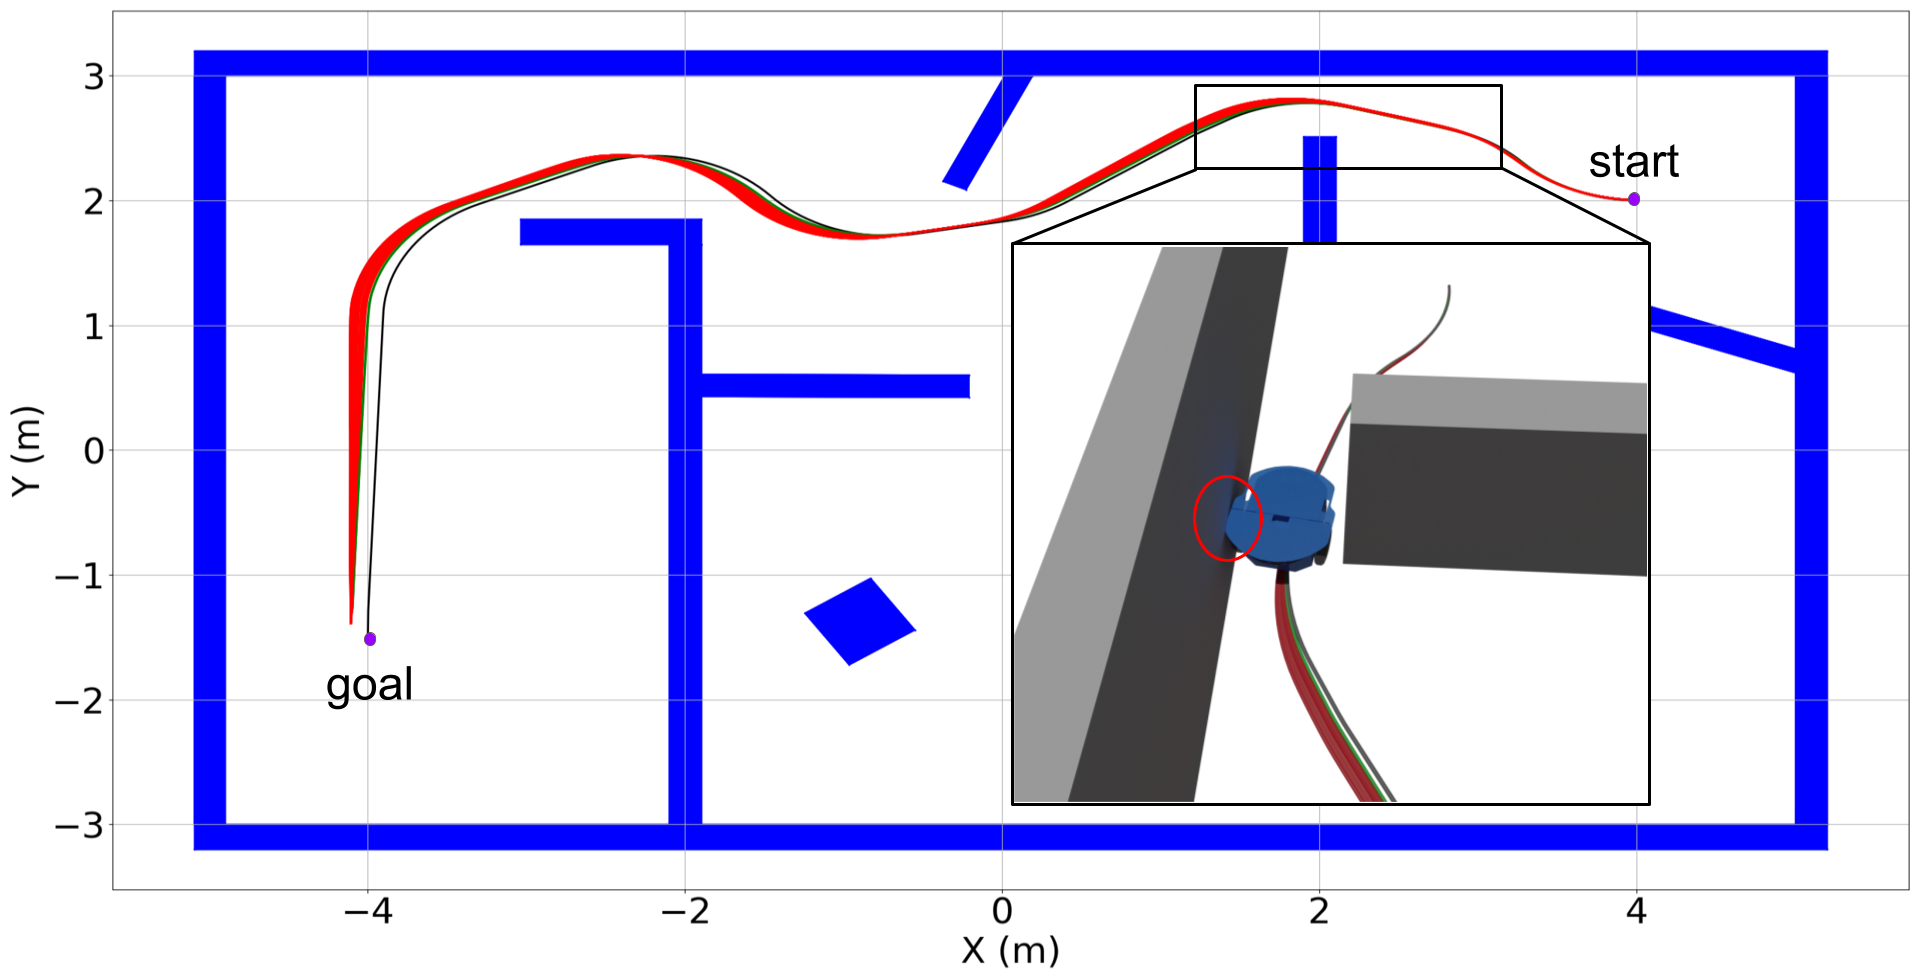
\includegraphics[width=0.9\linewidth]{figures/samp/non_robust_unic.png}
    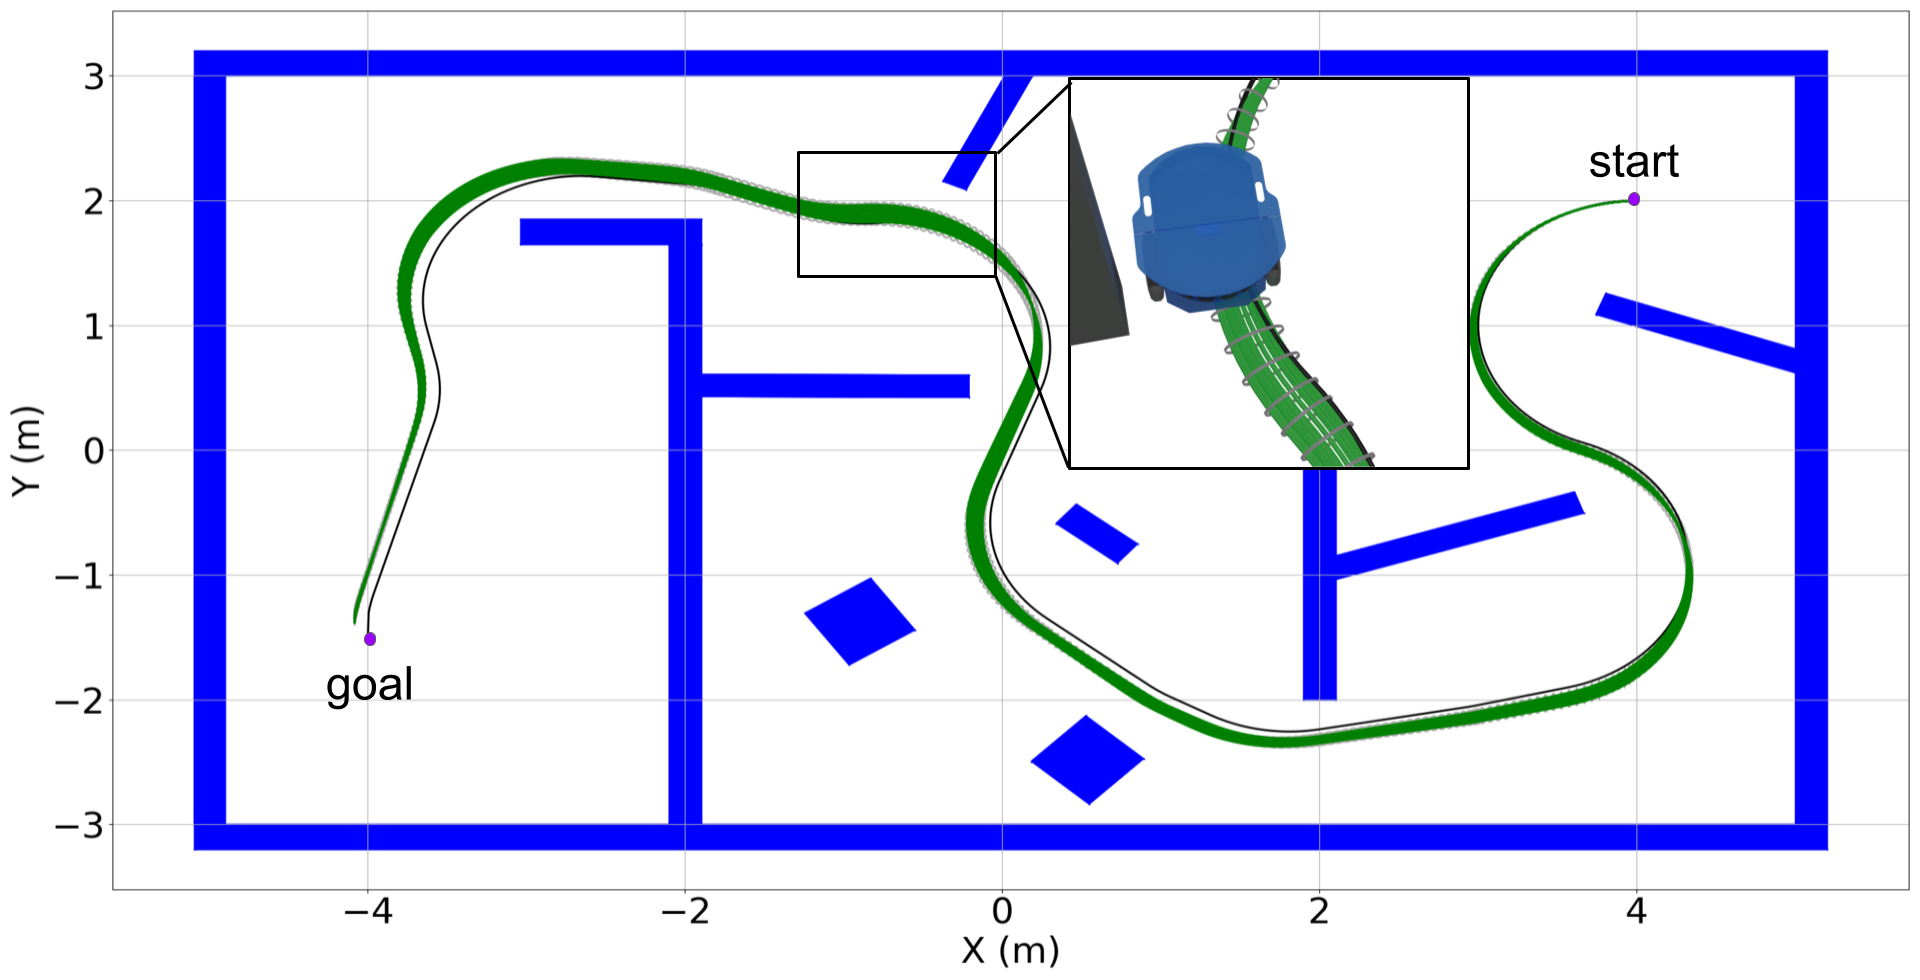
\includegraphics[width=0.9\linewidth]{figures/samp/robust_unic.png}
    \caption{Planned trajectory (black) produced by the \myglsentry{rrtstar} (top) and the \myglsentry{sarrt*} (bottom). 
    Simulated trajectories under uncertainty are displayed in green in the case of success, and in red in the case of a crash.}%
    \label{fig:robust_unic}%
\end{figure}

\begin{figure} [ht]
    \centering
    \includesvg[width=0.8\linewidth]{figures/samp/profiling_unic.svg} 
    \caption{Profiling of vanilla planners and robust \myglsentry{samp} variants, illustrating the contributions of various procedures to the total planning time over 1.000 iterations for the differential drive robot case.}%
    \label{fig:profiling_unic}%
\end{figure}

\subsubsection{Quadrotor robot}

\begin{figure} [htp]
    \centering
    \includesvg[width=0.7\linewidth]{figures/samp/sensi_cost_quad.svg} 
    \caption{Evolution of the sensitivity as a function of the planning time of a \myglsentry{sasst*} (green), and of \myglsentry{sarrt*} (red) for the quadrotor application.}%
    \label{fig:samp_quad_time}%
\end{figure}

\begin{figure} [htp]
    \centering
    \includesvg[width=0.8\linewidth]{figures/samp/profiling_quad.svg} 
    \caption{Profiling of vanilla planners and robust variants, illustrating the contributions of various procedures to the total planning time over 1.000 iterations for the quadrotor case.
    }%
    \label{fig:profiling_quad}%
\end{figure}

As explained in Section~\ref{sec:unified}, the set of \myglsentry{odes} must be solved at each algorithm iteration, one per iteration in the case of \myglsentry{sasst*} and at least tens or hundreds of times for the \myglsentry{sarrt*}.
Although this result in high but still manageable computation times for simple systems like the differential drive robot presented above, Figure~\ref{fig:samp_quad_time} highlights the intractability of such optimal planning techniques for the quadrotor case, which involve solving hundreds of \myglsentry{odes}.
Similar to the differential drive robot, the prohibitively long planning time is closely linked to the time spent solving the \myglsentry{odes}, as shown in Figure~\ref{fig:profiling_quad}, where the \emph{CC} procedure refers to standard collision checking or the robust feasibility check, \emph{Cost} is the trajectory cost computation procedure, \emph{NN} stands for the nearest neighbor search, \emph{Sampling} and \emph{LocalPlan} refer to the state space sampling and local trajectory planning respectively, \emph{Tree} procedure is in charge of the data structure management (e.g. pruning, child cost update, etc.), and finally \emph{ODEs} stands for the sensitivity and tubes computations.
Therefore, the frequency of \myglsentry{odes} solving must be further reduced, as even the \myglsentry{sasst*}, which performs only a single computation per iteration, faces challenges due to the tens of thousands of iterations required to adequately explore the space.

\section{Decoupled approach}\label{sec:decoupled}

As demonstrated in Section~\ref{sec:samp_simu}, the proposed \myglsentry{samp} variants are efficient for simple systems but face challenges with more complex ones, such as the quadrotor. 
Achieving effective state-space coverage and convergence to a solution requires thousands of iterations, each involving the resolution of \myglsentry{odes}. 
This creates a bottleneck for the method, particularly when solving the \myglsentry{odes} requires tens of milliseconds for hundreds of time steps, as is common in complex systems.
Therefore, this section introduces a decoupled approach that minimizes the frequency of solving the \myglsentry{odes}, offering a more efficient algorithm for complex systems, such as quadrotor, to generate robust trajectories with near-optimal sensitivity.

\subsection{Algorithms}

Since the cost function of Equation~(\ref{eq:cost_function}) corresponds to the integration of the sensitivity over the trajectory, it is then noticeable that starting from an initial (near) time-optimal trajectory helps to produce initial solutions of rather good quality w.r.t. the sensitivity cost.
The proposed decoupled approach is based on a lazy sensitivity-aware variant, generally referred to as \gls{lazysamp}, that plans a robust (near) time-optimal trajectory.
This trajectory is then locally optimized for minimizing the cost function~(\ref{eq:cost_function}) via a robust variant of the `shortcut' technique classically used to smooth solutions of randomized planners~\cite{cShortcut}. 

\subsubsection{Lazy Sensitivity-Aware RRT* (LazySARRT*)}\label{sec:lazy_rrt*}

\begin{algorithm}[htp]
    \caption{LazySARRT$^* [q^{init}, q^{goal}]$}\label{alg:LazySARRT*}
    \begin{algorithmic}[1]
        \State $T \gets$ InitTree$({q^{init}, q^{goal}});$
        \While{\textbf{not} StopCondition$(T, {q^{goal}})$}  
            \State $q^{rand} \gets $Sample()$;$
            \State $q^{nearest} \gets$ Nearest$(T,{q^{rand}});$
            \State Extend$(T, q^{rand}, q^{nearest});$
            \State $Q_{sol} \gets CheckForSolution(T, q^{init}, q^{goal});$
            \If{$Q_{sol} \neq \emptyset$}
                \For { i = 0 and  i < size($Q_{sol}$)-1}
                    \State $S_0 \gets $GetNodeConditions$(Q_{sol}^{i});$
                    \State $\q_d \gets $LocalPlan$(Q_{sol}^{i}, Q_{sol}^{i+1});$
                    \State $\left \{\q_n, \u_n, \Rq, \Ru, S_F \right \}  \gets $SolveODEs$(\q_d, S_0);$
                    \If {\textbf{not} IsRobust$(\Rq,\Ru, \q_n, \u_n)$}
                        \State $T \gets $RobustReconnect$(T, Q_{sol}^{i});$
                    \EndIf
                \EndFor
            \EndIf
        \EndWhile
        \State \textbf{return} GetTrajectory$(T, q^{init}, q^{goal})$;
    \end{algorithmic}
\end{algorithm}

This subsection present the \gls{lazysarrt*}, as a particular instance of \myglsentry{lazysamp}, that plans a robust (near) time-optimal trajectory.
The algorithm not only provides a (near) time-optimal trajectory but also ensures that the resulting trajectory is collision-free w.r.t. the state uncertainties and also that control inputs remain in their allowed bounds.
However, as highlighted in Section~\ref{sec:unified}, the number of \myglsentry{odes} computation within the \myglsentry{rrtstar} must remain as limited as possible to avoid a too long computing time. 
For this reason, trajectory robustness is checked in a lazy way, only when a better solution is found, and reconnecting the nodes optimally if necessary.
The lazy process is achieved as described in~\cite{cLazy1,cLazy2}, with the addition of maintaining a set of non-robust parents ($Q_{collide}$) for each node.
Consequently, unlike the \myglsentry{samp} methods described in Section~\ref{sec:samp}, the tree built by the lazy variant is not inherently robust; only the final solution meets the robustness requirements.

Algorithm~\ref{alg:LazySARRT*} provides the pseudo-code of the \myglsentry{lazysarrt*} variant.  
The first stage applies the unmodified \myglsentry{rrtstar} (line 1-5) where the Extend procedure performs the standard collision checking (i.e. without uncertainty tubes), optimal connection, and rewiring phase for the given sample  $q^{rand}$ as in~\cite{cRRTstar}.
The algorithm then verifies at each iterations whether a new, lower-cost solution has been discovered. 
If a better solution is identified, the set of nodes $Q_{sol}$, which enables the reconstruction of this solution, is retrieved (line 6).

Next, for each local trajectories between two consecutive nodes in this set, the \myglsentry{odes} are solved, and the uncertainty tubes computed (line 9-11).
The algorithm then verifies the robust feasibility of the local trajectory using a robustness test w.r.t. obstacles but also control inputs saturation. 
If a local trajectory is found to be non-robustly feasible, all nodes in the tree connected to $Q_{sol}^i$ are disconnected and reconnected using the RobustReconnect procedure (line 13).

The RobustReconnect procedure may differ depending on the specific \myglsentry{lazysamp} variant used (see Chapter~\ref{chap:sampNN}). 
In the case of \myglsentry{lazysarrt*}, where maintaining an optimal tree is required, it operates as follows:
\begin{itemize}
    \item For all tree nodes, a set of robust infeasible parent $Q_{collide}$ is maintained. 
    The RobustReconnect procedure starts by adding $Q_{sol}^i$ in the set of infeasible parents of $Q_{sol}^{i+1}$ (i.e. $Q_{sol}^i$ will no longer be considered as a potential parent for the node $Q_{sol}^{i+1}$).
    \item Then, all the nodes of the tree from $Q_{sol}^i$ are disconnected, and for each of them, the vanilla Extend procedure is executed considering their associated $Q_{collide}$ set.
    As in the standard \myglsentry{rrtstar}, an optimal re-connection phase is first attempted.
    All nodes must be evaluated for optimal reconnection, as the non-robust invalid edge may be reconnected, but its child nodes could potentially find improved connections.
    \item If no re-connection is found for a node, then the node is deleted from the tree. 
    Otherwise, the rewiring phase is carried out considering the $Q_{collide}$ set.
\end{itemize}

The output of \myglsentry{lazysarrt*} is a (near) time-optimal trajectory that is feasible in terms of both collision avoidance and actuator saturation, accounting for uncertainties.
It is however not optimized in terms of the sensitivity. 
Therefore, its robustness can be further improved.

\subsubsection{Sensitivity-Aware Shortcut}

\begin{algorithm}[htp]
    \caption{SAShortcut [$\q_{d,SARRT^*}$]}\label{alg:SAshortcut}
    \begin{algorithmic}[1]
        \State $\{\q_{d,best}, cost_{best}\} \gets \{\q_{d,SARRT^*}, $Cost$(\q_{d,SARRT^*}) \};$
        \State $q_d^{init} \gets \q_{d,best}^0; q_d^{goal} \gets \q_{d,best}^F;$
        \While{\textbf{not} StopCondition$()$} 
            \State $\{q_d^{1}, q_d^{2}\} \gets$ SampleOnTraj$(\q_{d,best});$
            \State $\q_{d,shct} \gets $LocalPlan$(q_d^{1}, q_d^{2});$
            \If{CollisionFree$(\q_{d,shct})$}
                \State $\q_{d,start} \gets $LocalPlan$(q_d^{init}, q_d^{1});$
                \State $\q_{d,end} \gets $LocalPlan$(q_d^{2}, q_d^{goal});$
                \State $\q_{d,new} \gets \q_{d,start}+\q_{d,shct}+\q_{d,end};$
                \State $S_0 \gets $GetNodeConditions$(q_d^{init});$
                \State $\{\q_n, \u_n, \Rq, \Ru, S_F\}  \gets $SolveODEs$(\q_{d,new}, S_0);$
                \State $cost_{new} \gets $Cost$(\q_{d,new});$
                \If{CostBetterThan$(cost_{new}, cost_{best})$}:   
                    \If {IsRobust$(\Rq,\Ru, \q_n, \u_n)$}
                        \State $\{\q_{d,best}, cost_{best}\} \gets \{\q_{d,new}, cost_{new}\};$
                    \EndIf
                \EndIf
            \EndIf
        \EndWhile
    \State \textbf{return} $\q_{d,best}$
    \end{algorithmic}
\end{algorithm}

In order to improve the sensitivity-based cost function, a local optimization is performed using a simple robust sensitivity-aware variant of the 'shortcut' smoothing algorithm~\cite{cShortcut}, called \gls{SAshortcut} and described in Algorithm~\ref{alg:SAshortcut}. 
A more detailed discussion regarding the robust sensitivity-aware local optimization can be found in Chapter~\ref{chap:sampNN}.

The algorithm is first initialized with the robust trajectory resulting from the \myglsentry{lazysarrt*} presented above (line 1).
It is important to note that the robustness of the initial trajectory is a crucial assumption, as the \myglsentry{SAshortcut} algorithm does not guarantee the generation of a robust trajectory if the initial trajectory is not robust.
Nevertheless, the algorithm preserves this robustness throughout its local optimization process.
Then, the algorithm randomly samples two states $\{q_d^{1}, q_d^{2}\}$, along the current best trajectory (line 4).
Next, it computes the local trajectory between the two samples $\q_{d,shct}$ (line 5).
To minimize the frequency of solving the \myglsentry{odes}, a lazy approach is employed.
First, the algorithm ensures that the proposed shortcut is collision-free (line 6). 
Unlike the classical shortcut method, which compares only the costs of the original and proposed trajectory segments, the entire trajectory is reevaluated to incrementally compute the sensitivity cost (lines 7–12).
It is important to note that both the cost and uncertainty tubes are derived from the \myglsentry{odes}. 
To avoid redundant computations, the \myglsentry{odes} are solved before performing the cost comparison.
Finally, if the new solution has a lower sensitivity cost (line 13), then a robust feasibility check is performed before updating the trajectory portion in case of success (line 14-15).

\subsection{Simulation results}
\subsubsection{Differential drive robot}

\input{figures/tables/lazySAMP_unic.tex}

\begin{figure}[htp]
    \centering
    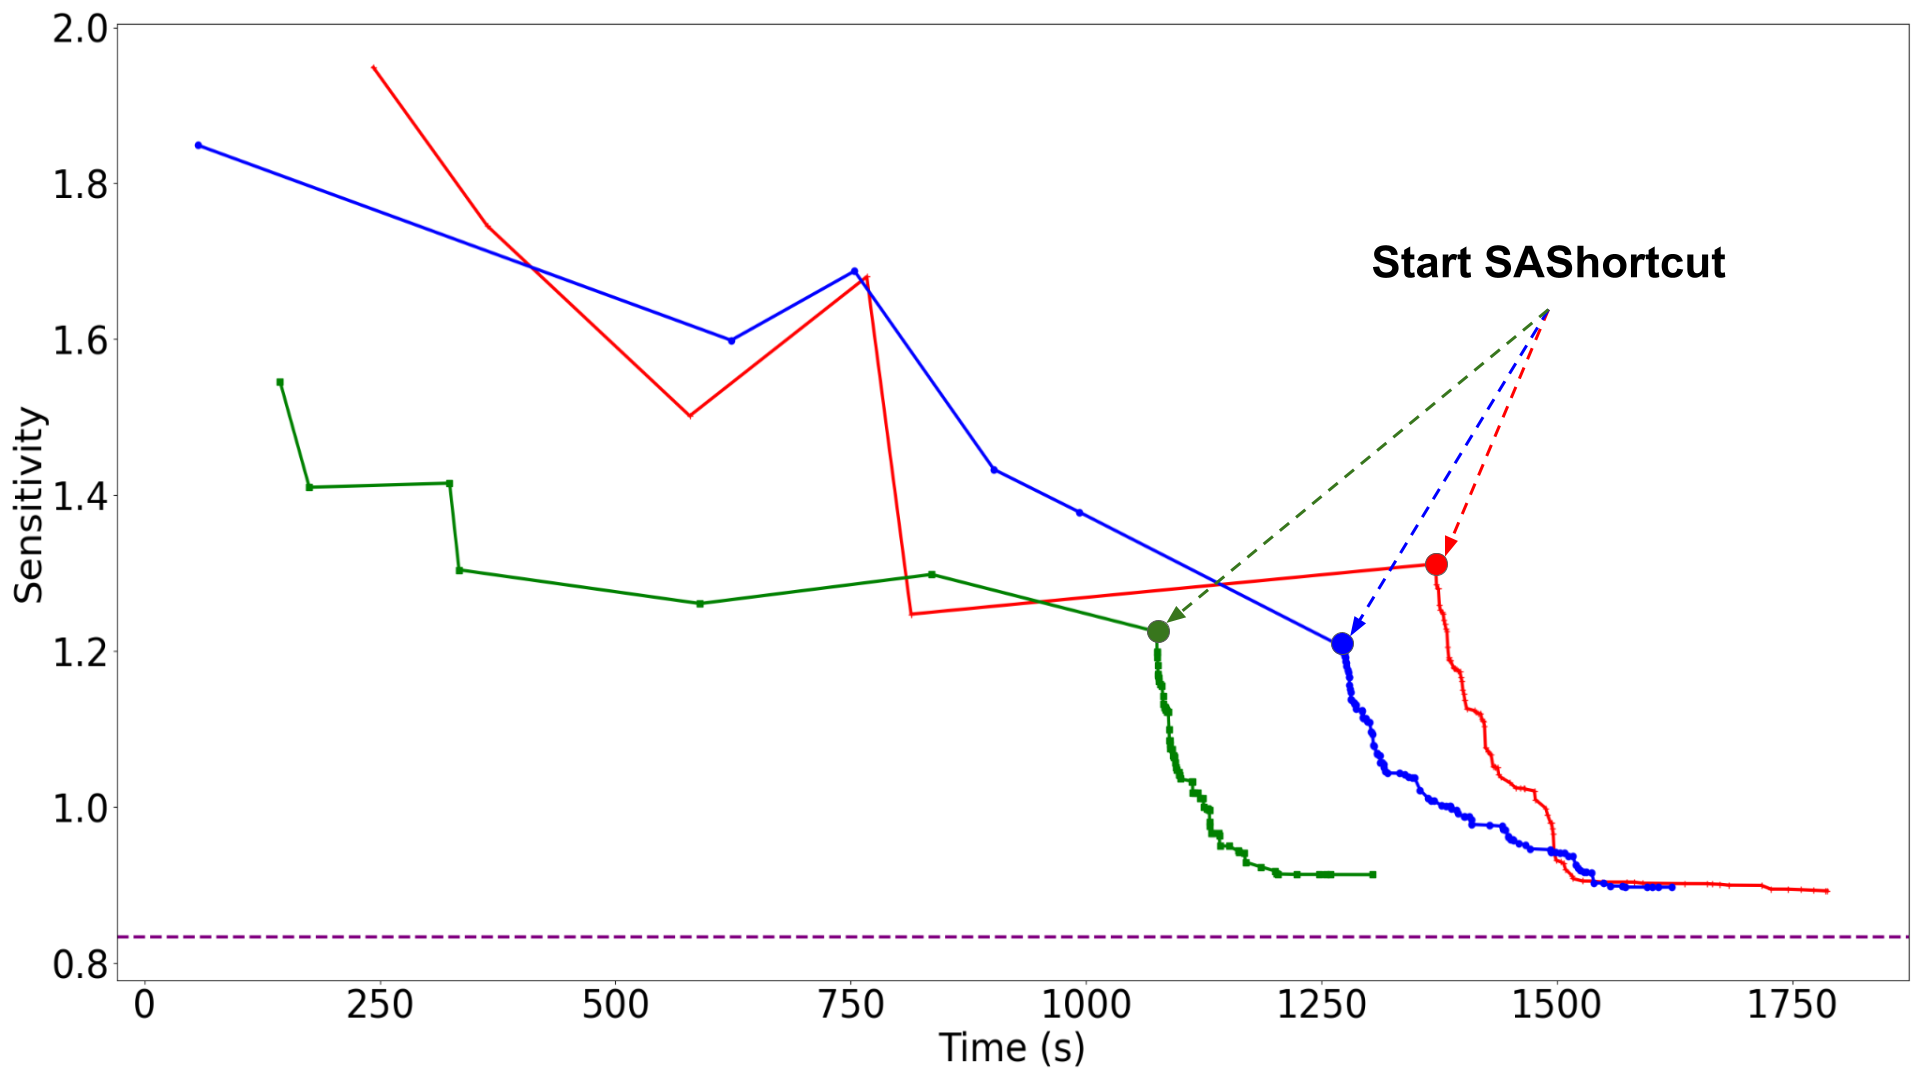
\includegraphics[width=0.7\linewidth]{figures/samp/sensi_cost_unic.png}
    \caption{Trajectory cost resulting of the decoupled approach (red, green, blue) for the differential drive robot, the dashed purple cost correspond to the sensitivity-optimal reference trajectory found by the \myglsentry{sasst*}.}
    \label{fig:sensi_cost_unic}
\end{figure}

The decoupled approach is tested for the same differential drive robot settings as in Section~\ref{sec:samp_simu} where the \myglsentry{lazysarrt*} produces robust (near) length-optimal trajectories.
Table~\ref{tab:lazySAMP_unic} presents the average computation times over 10 runs for \myglsentry{sasst*} and the two core procedures of the proposed decoupled approach (\myglsentry{lazysarrt*}, \myglsentry{SAshortcut}), demonstrating a time savings of only 29.56\%.
The average cost find by the decoupled approach is of $0.925 \pm 0.032$ against $0.894 \pm 0.046$ for the \myglsentry{sasst*}, denoting a sub-optimallity of $3.47\%$.

The process is illustrated by the Figure~\ref{fig:sensi_cost_unic} where it is worth noting that during the \myglsentry{lazysarrt*} planning process, trajectory length optimization leads to a reduction in sensitivity cost, even though this was not the primary objective. 
This supports the choice of a (near) length-optimal trajectory as the initial guess for \myglsentry{SAshortcut} and validates the use of a length-based metric as the state-space metric when optimizing sensitivity within the \myglsentry{sarrt*} and \myglsentry{sasst*} methods discussed in Section~\ref{sec:samp_simu}.

\subsubsection{Quadrotor robot}

\paragraph{Setup}

To further evaluate the effectiveness of the decoupled approach, the quadrotor model described in Section~\ref{sec:quad_model} is used with the following set of uncertain parameters: $\p = [k_{f}, \, k_{\tau}, \, x_{cx}, \, x_{cy}]$, where $k_{f}$ and $k_{\tau}$ are coefficients associated with the dynamics of the propellers, and $x_{cx}$ and $x_{cy}$ are the location of the \myglsentry{com} in the $x$-axis and $y$-axis of the quadrotor body frame, which may be uncertain due to the presence of on-board sensors for example.
The values of this vector considered in the simulations are either $\delta\p_{low} = [10\% , 10\% ,  5cm , 5cm]$ or $\delta\p_{high} = [25\%, \, 25\%, \, 10cm, \, 10cm]$, where the first two components are a percentage of their associated nominal values. 
Note that the tubes computed from $\delta\p_{low/high}$ remain an approximation, but that are accurate enough for well-chosen $\delta\p$ values. 
Therefore, in this differential drive robot application, $\bPi \in \mathbb{R}^{13\times4}$, and $\bTheta \in \mathbb{R}^{4\times4}$.
As a result, the computations necessary to find the uncertainty tubes involve solving 68 \myglsentry{odes}.
The uncertainty tubes considered for this application are defined as $\Rq = [r_x, \, r_y, \, r_z]^T \in \mathbb{R}^3$, representing the uncertainty tubes along the \{x,y,z\}-axes of the state respectively, and $\Ru = [r_{u1}, \, r_{u2}, \, r_{u3}, \, r_{u4}]^T \in \mathbb{R}^4$, representing the uncertainty tubes along the four control input space axes.
Finally, the controller gains are set to $\boldsymbol{k}_{x} = [20.0, \, 20.0, \, 25.0]^T$, $\boldsymbol{k}_{v}= [9.0, \, 9.0, \, 12.0]^T$, $\boldsymbol{k}_{R}=[4.6, \, 4.6, \, 0.8]^T$, and $\boldsymbol{k}_{\omega}=[0.5, \, 0.5, \, 0.08]^T$, and the control inputs limits are set to $\u_{max} = [10.000, \, 10.000, \, 10.000, \, 10.000]^T$, corresponding to the maximum squared rotor speed expressed in (rad.s$^{-1})^2$.

\paragraph{Planning}

The performances of the decoupled approach are evaluated in three different environments, also considering different parametric uncertainties.
The local planning method used is the kinospline local planner (see Section~\ref{sec:kinosplines}), which rely on an efficient state-space quasi-metric, as defined in~\cite{cKino}, for the distance function.
In the 2D environments (U-shape and 2-Way), the quadrotor is forced to evolve on a plane by generating kinosplines only between samples within the plane and by not allowing displacements along the z-axis.

The sensitivity-optimal trajectories used as references to evaluate the decoupled approach, are computed using the \myglsentry{sasst*} algorithm with hyperparameters selected according to the guidelines provided in~\cite{cSST}: $N_0 = 10000$, $\delta_s = 3$, $\delta_{BN} = 5$, and $\xi = 0.9$.
For the maximum local distance, $d_{max}$ is set to 1.0.
Finally, the \myglsentry{odes} and the robust feasibility check are performed using a time step of 0.05s.

\paragraph{Results}

\newcolumntype{C}[1]{>{\centering\arraybackslash }b{#1}}
\begin{table*}[t]
    \centering
    \begin{tabular}{|C{0.185\linewidth}||C{0.095\linewidth}|C{0.12\linewidth}|C{0.12\linewidth}|C{0.09\linewidth}|}
     \hline
      & U-shape & 2-Way$_{low}$ & 2-Way$_{high}$ & 3D \\
     \hline
     \hline
     Time \myglsentry{sasst*}  (s) & 7221 & 16615 & 23194 & 26875 \\
     \hline
     Time \myglsentry{lazysarrt*} (s) & \textbf{673} \quad $\pm$ 247& \textbf{2506} \quad\quad $\pm$ 305& \textbf{3271} \quad\quad $\pm$ 440& \textbf{2388} \quad $\pm$ 342\\
     \hline
     Time \myglsentry{SAshortcut} (s) & \textbf{453} \quad $\pm$ 191& \textbf{374} \quad\quad $\pm$ 173& \textbf{753} \quad\quad $\pm$ 104& \textbf{577} \quad $\pm$ 229\\
     \hline 
     Decoupled approach time gain (\%)  & 84.4 & 82.7 & 82.6 & 89.0 \\
     \hline
     \hline
      Cost \myglsentry{sasst*} & 0.317 & 0.292 & 5.127 & 0.510 \\
     \hline
      Cost decoupled approach & \textbf{0.324} \quad $\pm$ 0.003& \textbf{0.298} \quad $\pm$ 0.002& \textbf{5.274} \quad\quad $\pm$ 0.041& \textbf{0.523} \quad $\pm$ 0.071\\
     \hline
      Sub-optimality decoupled approach (\%) & 2.21 & 2.01 & 2.87 & 2.55 \\
     \hline
    \end{tabular}
    \caption{
    \label{tab:lazySAMP_quad}
    Average values of costs and computing times for the different methods in several environments.
    Standard deviations are provided for the SAMP results only as the SST$^*$ results do not contain enough runs.
    }
\end{table*}

Table~\ref{tab:lazySAMP_quad} gathers the average computing times of \myglsentry{sasst*} and of the two core procedures of the proposed decoupled approach (\myglsentry{lazysarrt*}, \myglsentry{SAshortcut}), as well as the average final cost found by \myglsentry{sasst*} and \myglsentry{SAshortcut}. 
The mean values associated with \myglsentry{sasst*} were obtained over 3 runs (due to the very high computing time) while those associated with the proposed decoupled approach are averaged over 10 runs.

\paragraph{2D U-Shape Environment} 

\begin{figure}[htp]
    \centering
    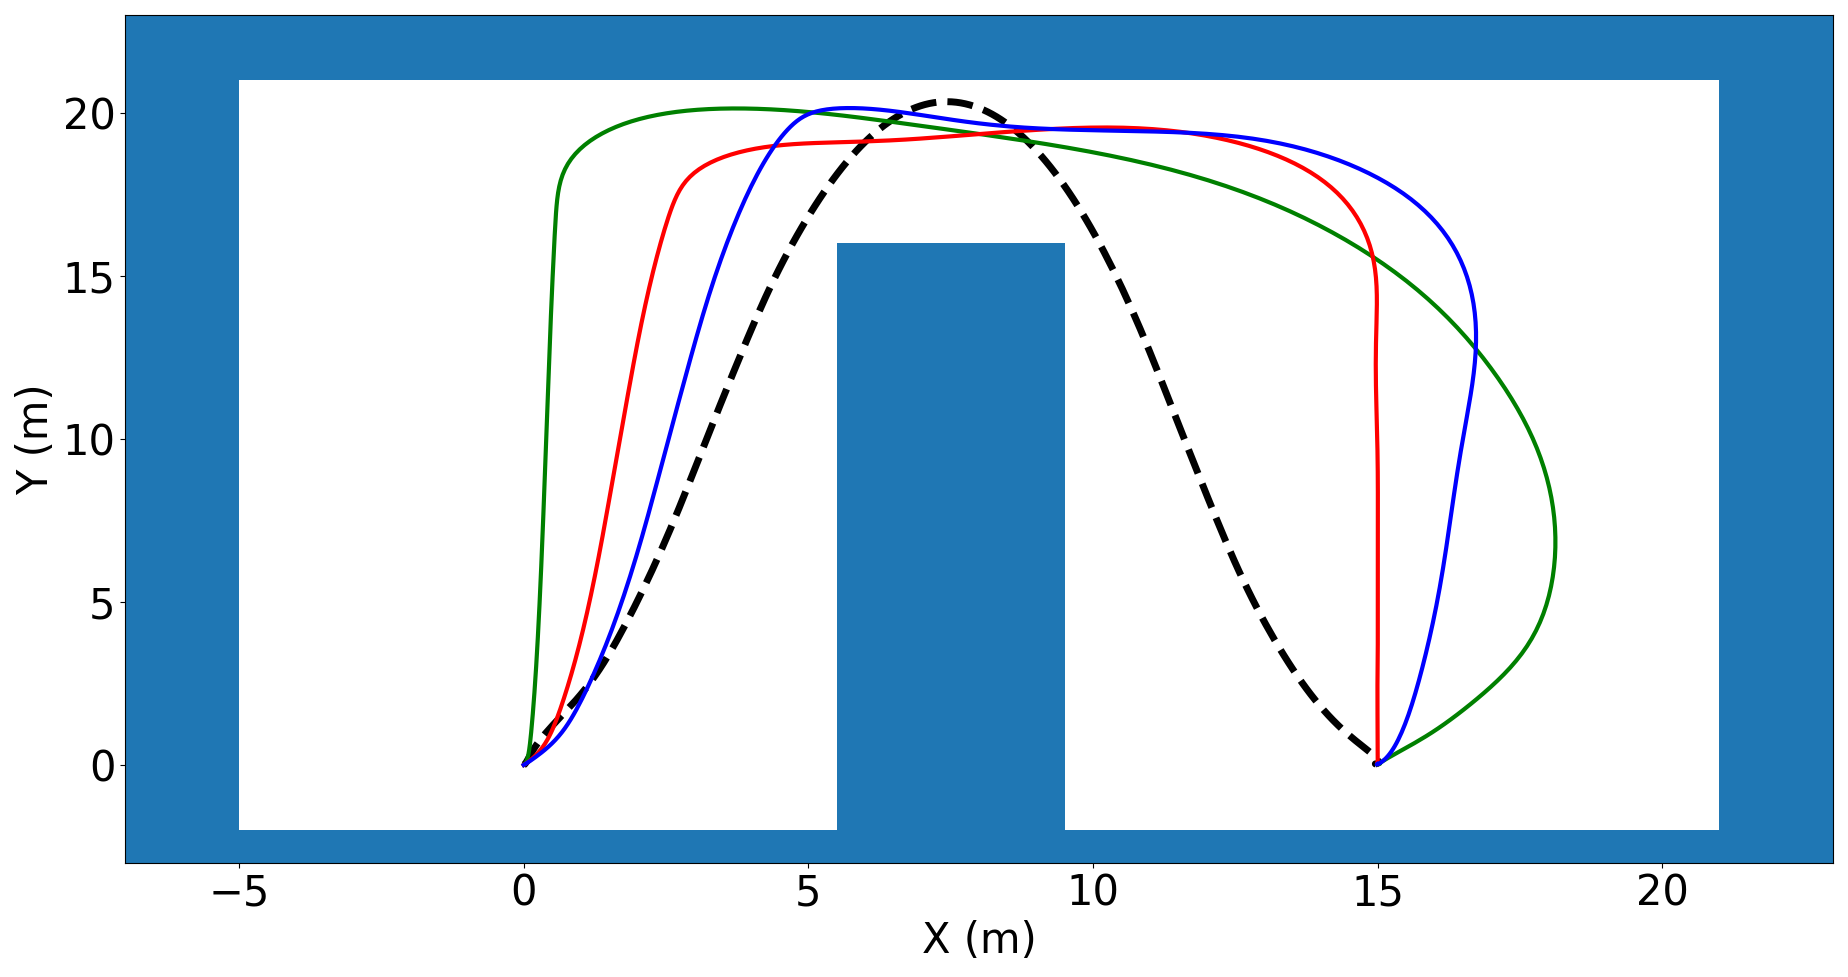
\includegraphics[width=0.7\linewidth]{figures/samp/U_shape_3in1_before.png}
    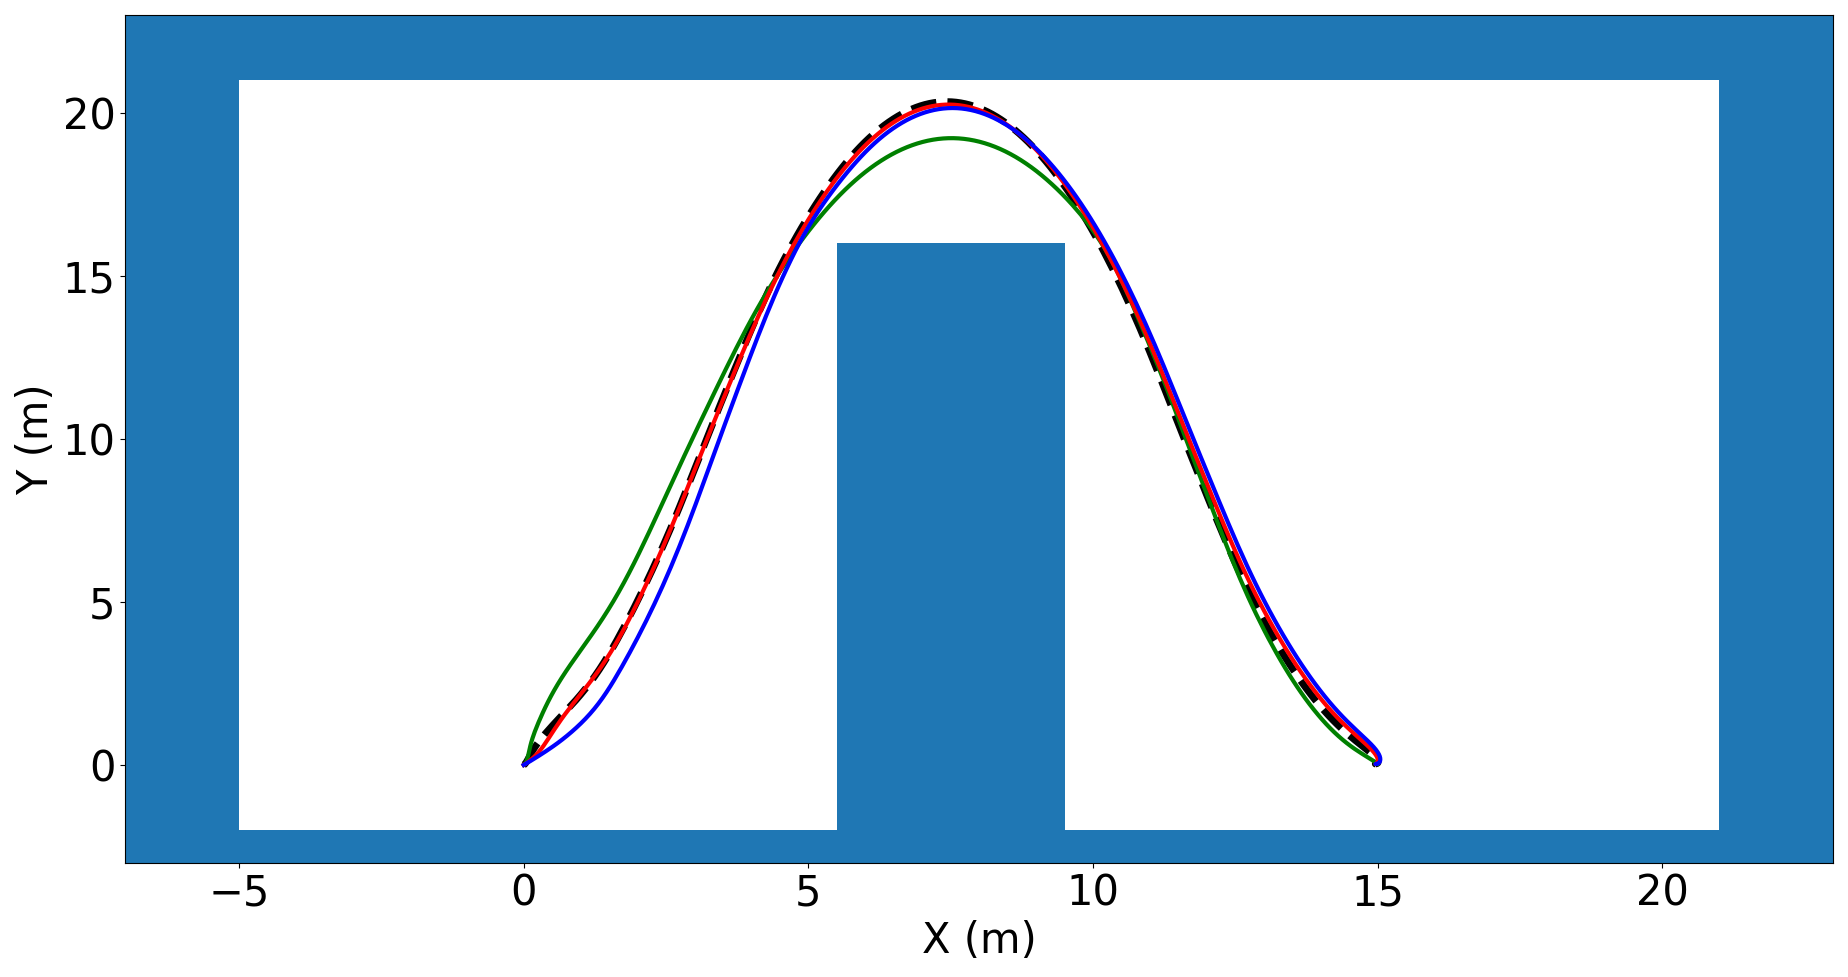
\includegraphics[width=0.7\linewidth]{figures/samp/U_shape_3in1_after.png}
    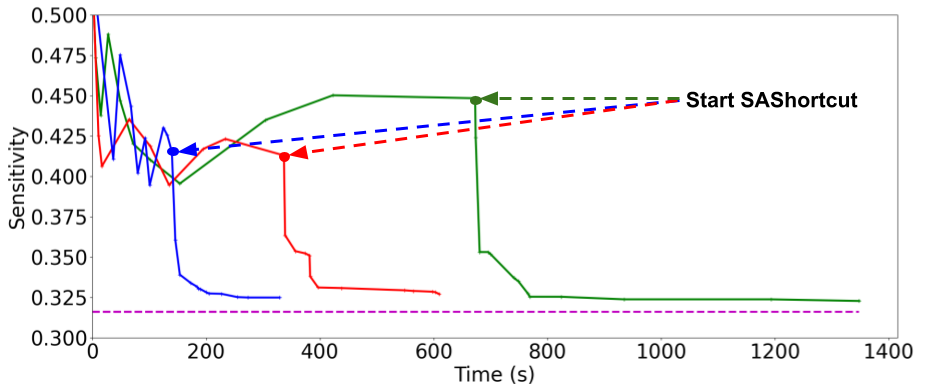
\includegraphics[width=0.7\linewidth]{figures/samp/U_shape_3in1_sensi.png}
    \caption{Three trajectories (red, green, blue) produced by \myglsentry{lazysarrt*} (top), and the three trajectories resulting from \myglsentry{SAshortcut} (middle), with the evolution of their respective sensitivity (bottom). 
    The dashed black trajectory (top, middle) and the dashed purple cost (bottom) correspond to the sensitivity-optimal reference trajectory found by the \myglsentry{sasst*}.}
    \label{fig:U_shape}
\end{figure}

Figure~\ref{fig:U_shape} shows how the decoupled approach is able to produce solutions that mimic the optimal one found by the \myglsentry{sasst*} in the so called U-shape environment considering the $\delta\p_{low}$ parametric uncertainty vector.
Furthermore, according to the results shown in Table~\ref{tab:lazySAMP_quad} and in Figure~\ref{fig:U_shape}, \myglsentry{SAshortcut} produces solutions with sensitivity costs close to the optimal reference found by \myglsentry{sasst*}. 
Also note the huge time saving of the proposed method compared to the \myglsentry{sasst*}.
Additionally, it is again worh to note that during the \myglsentry{lazysarrt*} planning, trajectory length optimization results in a reduction of the sensitivity cost, further corroborating the observations made in the differential drive robot application.

Finally, note that the average computing time of \myglsentry{lazysarrt*} in this case is low compared to the other environments. 
This is mainly due to the fact that in this case the time-optimal trajectory is far from the obstacles and therefore few re-connections via the \myglsentry{lazysarrt*} RobustReconnect procedure are performed when extending the tree.

\paragraph{2D 2-way Environments} 

\begin{figure}[htp]
    \centering
    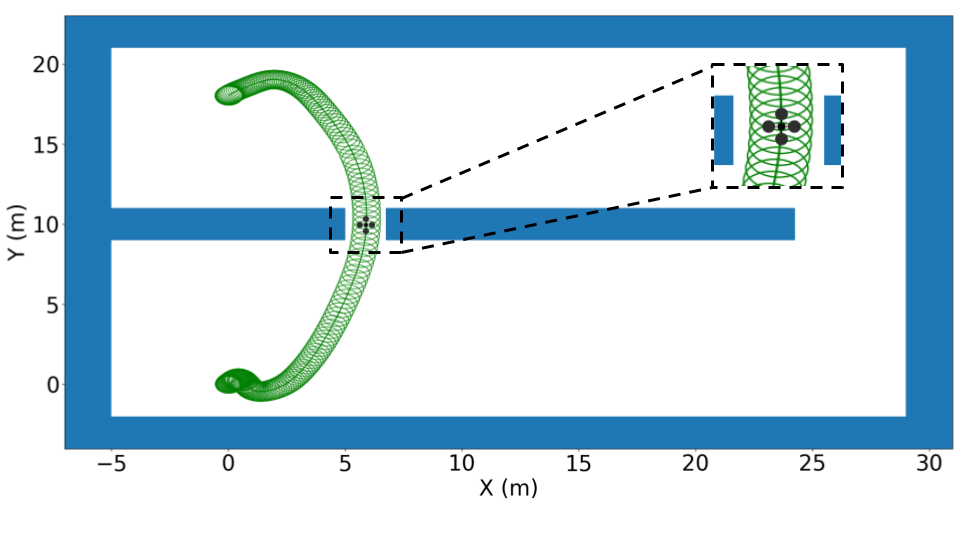
\includegraphics[width=0.7\linewidth]{figures/samp/Contribution-example1.png}
    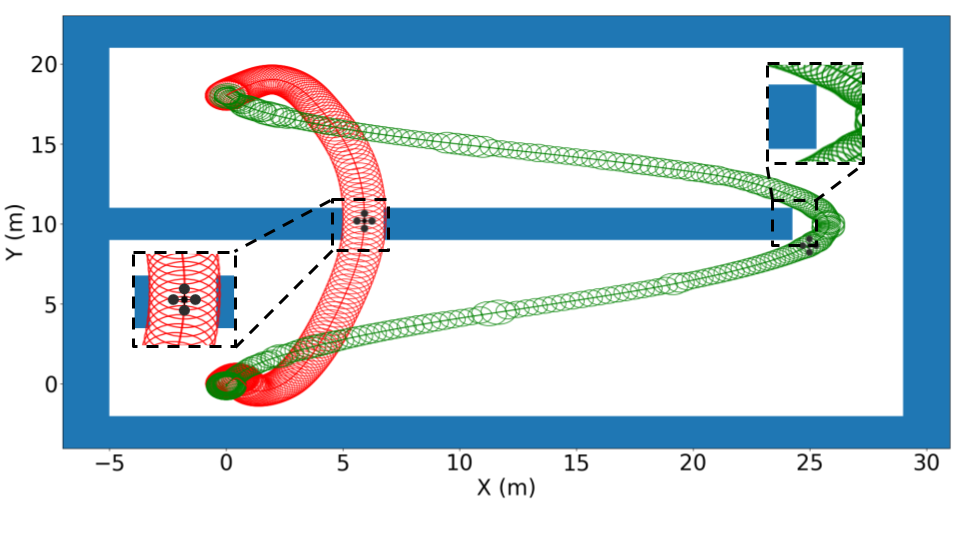
\includegraphics[width=0.7\linewidth]{figures/samp/Contribution-example2.png}
    \caption{Solutions with their uncertainty tube (in green) computed by the decoupled approach between the same start/goal states of a quadrotor dynamical model for small/high parameters uncertainties (top/bottom, respectively)}
    \label{fig:2way}
\end{figure}

This environment referred to Figure~\ref{fig:2way} where the two sets of uncertainties $\delta\p_{low}$ and $\delta\p_{high}$ are considered.

As shown in Figure~\ref{fig:2way}, in the presence of small uncertainties the decoupled approach produces a trajectory allowing to use the narrow passage. 
However, while considering large uncertainties, the non-robust time optimal trajectory, which goes through the narrow passage, cannot be taken as a collision is found by considering the uncertainty tube as shown in red in the Figure~\ref{fig:2way}.
Nevertheless, the approach is able to find the fastest trajectory apart from those passing through this passage.

In both cases the average cost of the solutions produced by the decoupled approach is close to that found by \myglsentry{sasst*} as shown in Table~\ref{tab:lazySAMP_quad}, where 2-Way$_{low}$ refers to the presence of small uncertainties and 2-Way$_{high}$ to the presence of large uncertainties.
The average computing time of the \myglsentry{sasst*} is equivalent in both cases as it is performed on exactly the same environment.
However, note that the average computing time of the \myglsentry{lazysarrt*} is longer than in the U-shape case because the time-optimal trajectories must pass through a location where many collisions may occur. 
Moreover, in the 2-Way$_{high}$ case the \myglsentry{lazysarrt*} computing time is longer than in the 2-Way$_{low}$ as even more non-robust trajectories are found.
This is because more iterations are needed before considering a neighborhood deprived of nodes passing through the narrow corridor.
Finally, on can note that the \myglsentry{SAshortcut} computing time remains of the same order of magnitude for both cases as that of the U-shape, and again the decoupled approach produces a solution much faster than \myglsentry{sasst*}.

\paragraph{3D Environment} 

\begin{figure}[htp]
\centering
    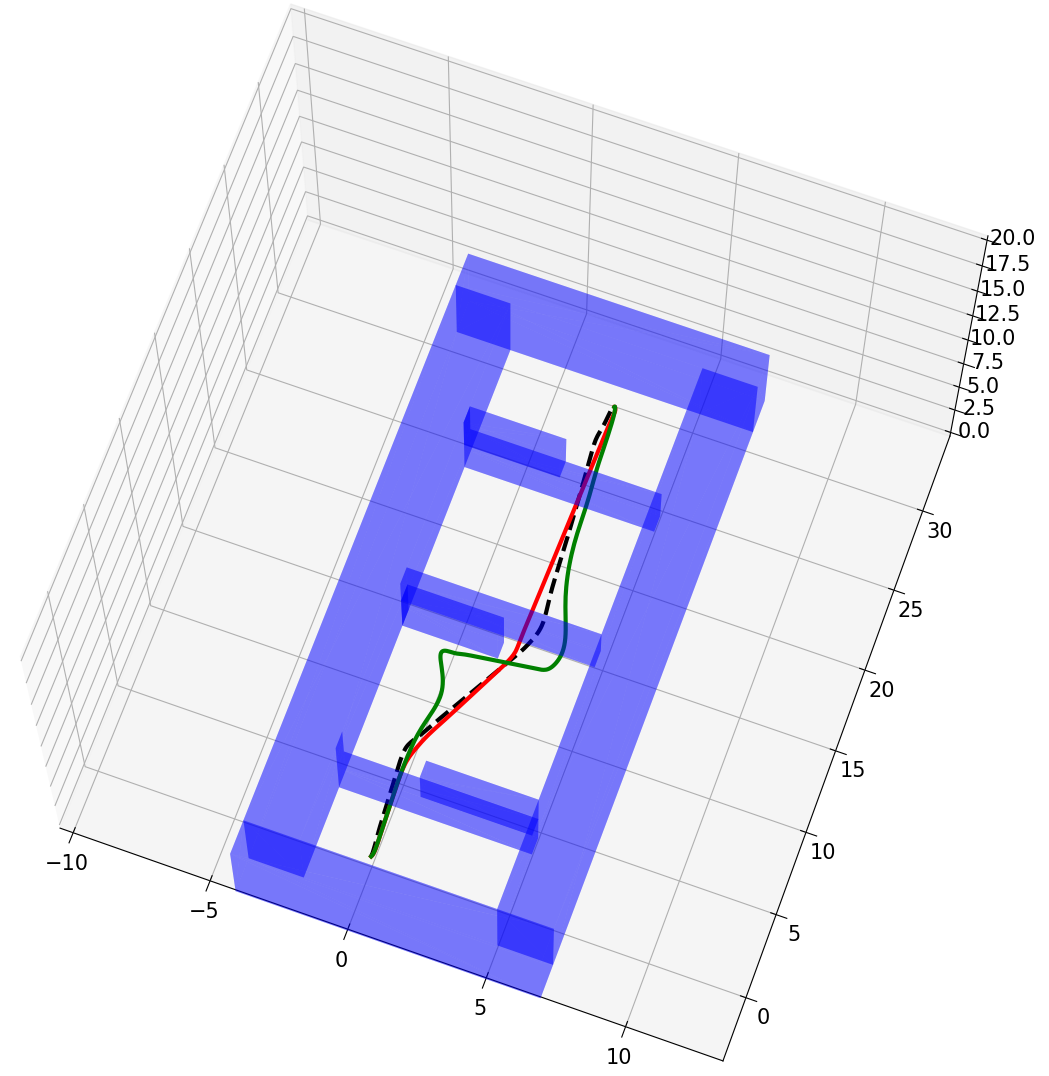
\includegraphics[width=0.7\linewidth]{figures/samp/3D_full_view.png}
    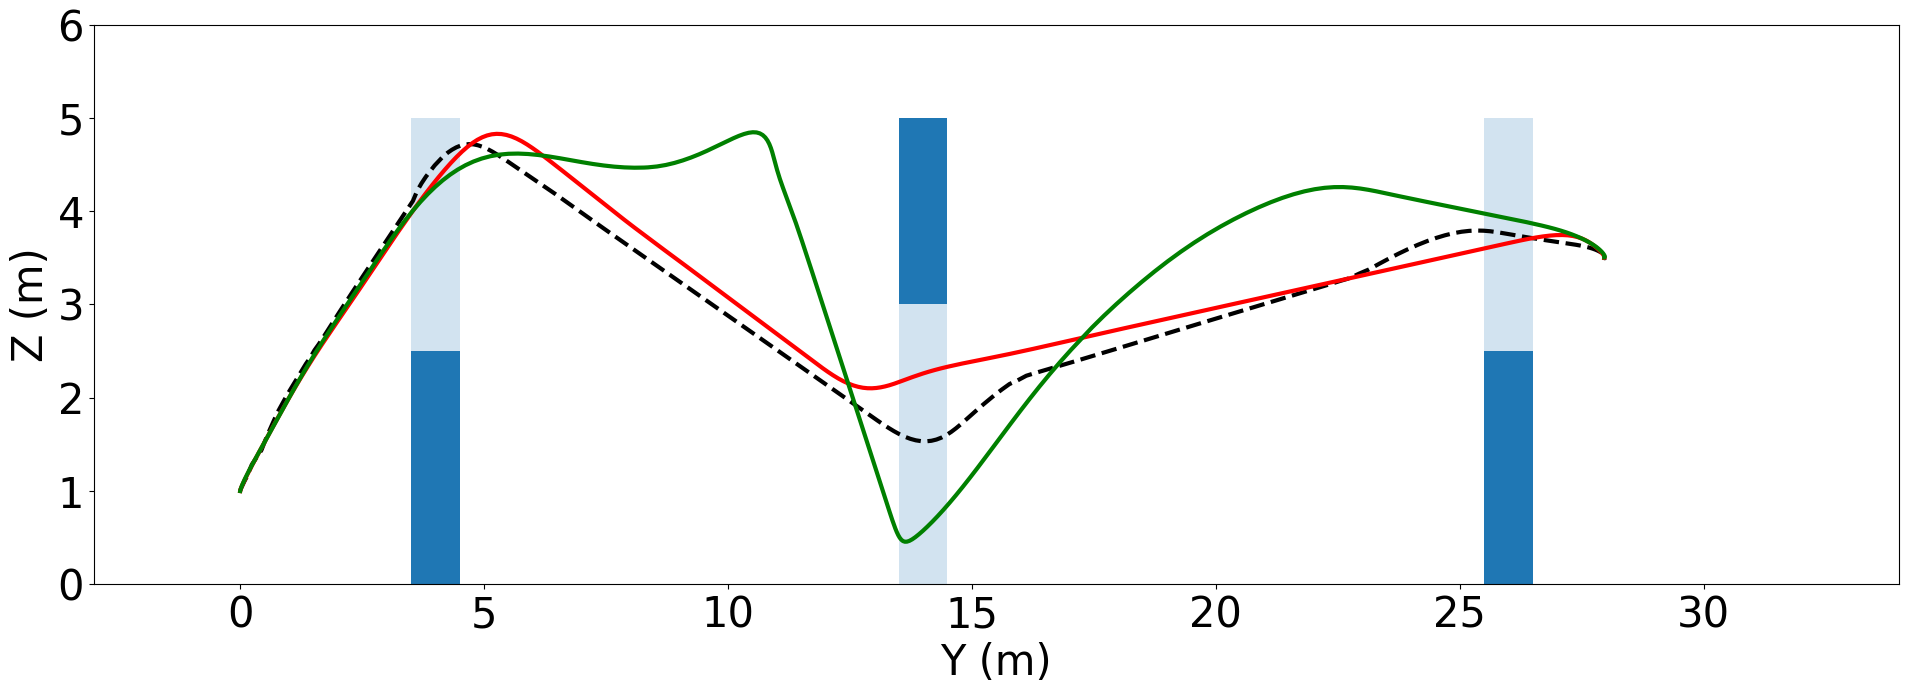
\includegraphics[width=0.7\linewidth]{figures/samp/3D_ZYprofile.png}
    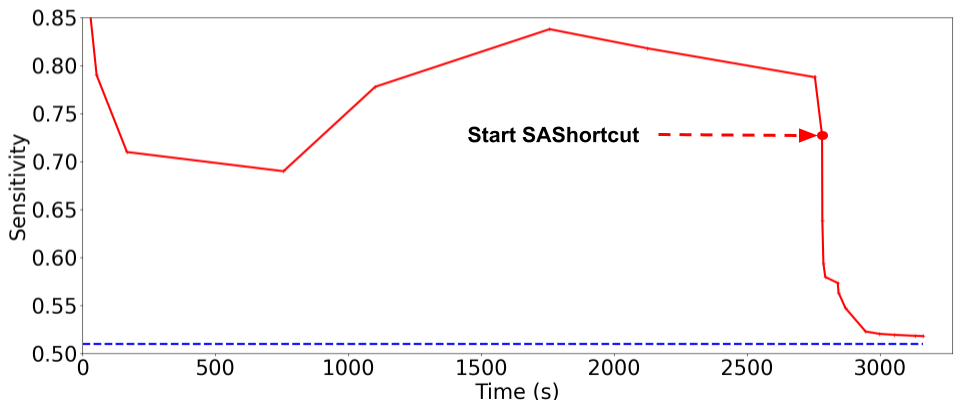
\includegraphics[width=0.7\linewidth]{figures/samp/3D_sensi.png}
    \caption{Trajectories produced by \myglsentry{lazysarrt*} (green), \myglsentry{SAshortcut} (red), and \myglsentry{sasst*} (dashed black) in a 3D environment (top). 
    A profile view along the YZ plane is given (middle) as well as the evolution of the sensitivity (red) and the optimal one found by the \myglsentry{sasst*} (dashed blue) (bottom).}
    \label{fig:3D}
\end{figure}

The uncertainty set considered in this full 3D environment is $\delta\p_{low}$.
As shown in Figure~\ref{fig:3D}, once again the decoupled approach produces trajectories that mimic the optimal obtained by the \myglsentry{sasst*}.
It is interesting to note the impact of the \myglsentry{SAshortcut} procedure on the z component in addition to the impact on the \{x,y\} components already seen in the previous 2D environments.
The average computing time of the shortcut is similar to other environments according to Table~\ref{tab:lazySAMP_quad}.
Again, the proposed method produces a near-optimal trajectory much faster than conventional optimal planners.

Finally, it is worth noting that in all cases, the significantly higher planning time of the \myglsentry{sasst*} compared to the lazy approach indicates that robust constrained planning requires a greater number of iterations to achieve adequate state-space coverage and converge effectively.
Furthermore, the significantly greater time gains observed in the quadrotor application compared to the differential drive robot application indicate that minimizing the frequency of solving the \myglsentry{odes} for more complex systems is crucial for keeping computation times manageable when planning with sensitivity.

\section{Conclusion}\label{sec:concl}

This chapter presented the general methodology for generating robust, sensitivity-aware variants, referred to as \myglsentry{samp}. 
To address the challenge of robust sensitivity-optimal trajectory generation, two variants—\gls{sarrt*} and \gls{sasst*}—were introduced. While these methods were demonstrated to be effective for simpler systems, such as differential drive robots, they result in high computation times. 
For more complex systems, such as quadrotors, their direct application becomes computationally unmanageable.
This limitation is primarily due to the significant time required to solve the \myglsentry{odes}.

To overcome this bottleneck, a decoupled framework was specifically designed to manage global planning using sensitivity-based metrics more efficiently than traditional asymptotically optimal sampling-based tree planners. 
This chapter introduced the \gls{lazysamp} variants, which aim to reduce the frequency of solving the \myglsentry{odes}. 
Simulations demonstrated that while the decoupled approach yields near sensitivity-optimal trajectories with moderate time savings for simpler systems like differential drive robots, it achieves substantial time savings as system complexity increases.

However, computation times remain affected by the need to solve the \myglsentry{odes}, as the associated computational cost scales approximately linearly with their number.
Additionally, the decoupled approach generates trees that are not inherently robust; only the final trajectory satisfies robustness requirements, limiting the reusability of the generated plans for tasks such as re-planning.

To address these challenges, the next chapters of this thesis will explore learning techniques to accelerate \myglsentry{odes} computation and propose motion planning algorithms that leverage these learned models.